\documentclass[a4paper, 10pt, oneside]{article}

\usepackage[square, numbers, comma, sort&compress]{natbib}  % Use the "Natbib" style for the references in the Bibliography
\usepackage{verbatim} 
\usepackage[english]{babel}
\usepackage[utf8x]{inputenc}
\usepackage{graphicx}
\usepackage{multirow}
\usepackage{amsmath}
\usepackage{amssymb}
%\usepackage{cite}
\usepackage{booktabs}
\usepackage{epstopdf}
\usepackage{helvet} 
\renewcommand{\familydefault}{\sfdefault}
\usepackage{setspace}
\singlespacing % interlinea singola
\linespread{0.97}
\usepackage{color}
\usepackage[margin=2.5cm]{geometry}
\setlength{\parindent}{0pt}
% pacchetti aggiunti
\usepackage{comment}
\usepackage[export]{adjustbox}
\usepackage{subfigure}
%\usepackage{subcaption}
\usepackage{algorithm}
\usepackage{algorithmic}
\usepackage{amsfonts}
\usepackage{tabularx}
\usepackage{ltablex}
\usepackage{caption}


\usepackage{comment}

\usepackage{titling}
\renewcommand\maketitlehooka{\null\mbox{}\vfill}
\renewcommand\maketitlehookd{\vfill\null}

\usepackage{enumerate}
\usepackage{enumitem}
\usepackage[dvipsnames]{xcolor}
\newcommand*{\lorenzo}[1]{\textcolor{BurntOrange}{#1}}
\newcommand{\yasmin}[1]{\textcolor{Red}{#1}}
\newcommand{\giovanni}[1]{\textcolor{Blue}{#1}}


\title{RASD}
\author{Yasmin Awad, Lorenzo Carpaneto, Giovanni Dispoto}
\date{October 2020}

\begin{document}

\begin{titlepage}
\vspace*{\fill}
\begin{figure}[h!]
	\centering
	
\includegraphics[scale=0.5]{img/logopoli.png}
\end{figure}
\vspace{0.7em}
\begin{center}
	\Large \textbf{REQUIREMENTS ANALYSIS AND SPECIFICATION DOCUMENT}
\end{center}
\begin{center}
	\large Version 0.1
\end{center}
\begin{center}
	\large Version Date
\end{center}
\vspace{0.4em}
\begin{center}
	\Large \textbf{CLup – Customers Line-up } 
\end{center}
\vspace{-0.6em}
\begin{center}
	\normalsize Yasmin Awad, Lorenzo Carpaneto, Giovanni Dispoto
\end{center}
\vspace*{\fill}
\end{titlepage}

\normalsize


\newpage
\tableofcontents
\newpage

\section{Introduction}
\label{introduction}
%During the first part of Covid-19 pandemic was figured out the problem of manage people at grocery store. Outside these buildings roads were tons of people enquequed waiting for their turn to buy food, waiting time that could be spent in other activities.\textbf{CLup} allows to manage customers in order to minimize the time spent enqueued and also avoiding crowd inside the building, suggesting to people the right route in order to buy everything that they need, minimizing the flow inside ward departement. With CLup user can get a ticket and know at what time he should be at grocery store. The system is able to estimate time needed to user to get to grocery store and decide if he has to denqueued because doesn't have enough time for reach the position. Users can also book a slot of time to do their shopping. Using this option he need to provide to the system categories of items that he need or better the shopping list. This information is useful due to trace a correct path inside the building and also to load balancing areas. 
%\yasmin{ho provato a riscriverlo usando delle tue parti ma cambiando qualcosa}
The aim of the following documentation is to provide an overview of the project \textit{CLup - Customes Line-up}: an application whose goal is to allow customers to shop safely. During the Covid-19 pandemic a new problem arose in people's lives. In a world where social distance is no longer a choice but a necessity, it must be found a way to ensure the safety of people in their daily lives, even in places open to the public, such as grocery stores. Having to comply with health and hygiene regulations, grocery stores were not allowed to enter more than a certain number of people, with the result of the formation of very long queues outside the buildings. \textbf{CLup} allows to manage customers in order to minimize their time spent enqueued and avoiding crowd inside the building. With CLup the customer can line from home getting a ticket for the grocery store or book a specific time-slot for their needs. This documentation will illustrate a description of the system in terms of its functional and non-functional requirements. We are going to show goals, constraints, limits and principal use cases of the software. In practice, this document will provide a baseline for the project planning and estimation. The document is addressed to the developers, that will implement the requirements, and to the stakeholders, that will supervise the development process.

\subsection{Purpose}
\label{intro:purpose}
Customer Line-up (CL-up) is an application that aims to provide users with the tools to obtain access to Stores in a safe way, i.e. in order to avoid as much as possible the presence of external people (queues to enter) and to allow a number of internal people (number of people entered in the Store) lower than the allowed limit of each Store. All of this is made in order to comply as much as possible with any social distancing rules required by the competent authorities. To pursue this goal, the application provides a service both to the owners of the Stores (or whoever takes their place), that is the Managers, and to the buyers, that is the Customers. The application allows Users to create a different type of profile based on their identity, intended precisely as a Manager or Customer. Tools are provided to allow Customers to book for entry to the Stores remotely, that is for example from their own home, allowing a greater and more efficient social distancing.\\
\\
There are 2 ways offered by CLup to enter the Stores. The first concerns the collection of a Ticket that will put the Customer in a virtual queue to enter the Store on the same day. The application has also the role of alert the Customer in order to let him/her arrive in time for his/her turn, checking and keeping track of the state of the virtual queue. The second allows the Customer to book a Visit, that is an entrance to the Store on a specific day, for a specific shopping time-range. To book a Visit the Customer must also specify the category of groceries he/her is intended to buy, in order to assign him/her a map of the Store and an optimal route for his/her Visit. Furthermore, the application to be as efficient and simple as possible for users, will not only advise them a time of stay in the Store based on the user's data (that on his old time stays), but will also recommend which Stores are available or closest, always based on the user's habits.\\
\\
Regarding Managers, the application gives them the possibility to create a specialized profile in which they can request 'the creation of a Store', i.e. a virtual space that will be identified as their own Store, and through which Customers will be able to book Tickets or Visits to enter the shop itself. The Managers have in fact the task of inserting and helping the application in the creation and definition of the Store and it's rules. All this information may vary over time and must be kept up to date in order to guarantee a better service of the application.\\
\\
To guarantee entry only for Customers authorized to enter at that moment, whether they have requested a Ticket or a Visit, a QR code is checked. In practice, each Customer is associated with a QR code that will appear in his profile. At the entrance, this QR code must be scanned to verify that the Customer has actually booked the Visit for that moment or that it is his turn to enter via Ticket. Moreover, to allow the virtual queue to slide adequately, each QR code must be scanned also at the exit.\\
\\
Finally, to allow entry to those who do not have the adequate technology to use the application, a secondary option must be put in place, i.e. a fallback option. To allow anyone to collect a Ticket, we have opted for adding Totems at the entrance that have the ability to print Tickets.
\newline
\newline
\newline
\subsubsection{Goals}

\begin{enumerate}[label={G.\arabic{*}}]
    \item \label{goal:auth} Allow Guests to authenticate as Manager or Customer
    \item \label{goal:influx} Regulate the influx of people inside the Stores.
    \item \label{goal:effectiveQueue} Line up Consumers in an effective way, to avoid overcrowding and long waiting time.
    \item \label{goal:enqueue} Allow Customers to virtually line up for Stores requesting a Ticket from different locations and devices.
    \begin{enumerate}[label={\ref{goal:enqueue}.\arabic{*}}]
        \item \label{goal:enqueue:time} Alert Customers when to depart to arrive in time for their shopping.
        \item \label{goal:enqueue:fallback} Guarantee a paper ticketing service as a fallback option for people who do not have access to the required technology.
    \end{enumerate}
    \item \label{goal:visit} Allow Customers to virtually line up for Stores booking Visits to the Store in different days from different locations and devices.
    \begin{enumerate}[label={\ref{goal:visit}.\arabic{*}}]
        \item \label{goal:visit:path} Guide Customers inside the Store with a map, to shorten the time of their Visit and minimize contact with other other people.
        \item \label{goal:visit:notifications} Notify the Customer in day-time range, if possible Visits which might interest them are available.
    \end{enumerate}
\end{enumerate}

\pagebreak

\subsection{Scope}
\lorenzo{Maybe the shared are too specific. I just do not really understand the difference that should be from scopes "shared" and requirements}

\begin{flushleft}
Following the definition originally proposed by M. Jackson and P. Zave in 1995,
we will distinguish world phenomena that are event occurring in real world from machine
that is the software to be.
World and Machine comunicate with Shared Phenomena, they could be events controlled by the world and observed by the machine or events controller by machine and observed by the world.
\end{flushleft}

\begin{itemize}
    \item {\large \textbf{World}}
    \begin{enumerate}[label={S.W.\arabic{*}}]
        \item \textbf{People going into Stores}: people going to stores to buy grocery and other products.
        \item \textbf{Queue formation}: the creation of long lines outside the stores.
        \item \textbf{People moving inside Store}: people moving into store in order to find grocery
        \yasmin{
        \item \textbf{Need to buy}: circumstance in which someone needs to enter a Store in order to buy some groceries.
        \item \textbf{Social Distancing}: circumstance in which the society imposes certain hygienic, sanitary and social distancing rules.
        }
    \end{enumerate}
    \item {\large \textbf{Shared}}
    \begin{enumerate}[label={S.S.\arabic{*}}]
        \item A Customer can register and sign up to the Service
        %\item \textbf{Registration \& Login}: a user can sign-up or login if already registered to the application.
       % \item \textbf{Choosing user type}: a user can register to the app as a manager or a customer (\lorenzo{QR scanner?}). \lorenzo{Maybe delete this points} \giovanni{quote for deleting this} \yasmin{quoto}
       % \item \textbf{QR code}: each user has a unique QR code, generated from the app as soon as they register. \lorenzo{Maybe delete this points} \giovanni{quote Lorenzo} \yasmin{forse chiamarlo QR code association ?? o generation}
        % Ticket part
        \item A logged Customer can get a ticket to virtual line
       % \item \textbf{Get ticket}: a Customer can take a ticket to form a virtual line for a specific store. \yasmin{change in ".. can get a ticket to line up for a specific Store" ??}
        \item A Customer can take a ticket at the store 
        %\item \textbf{Get paper ticket}: a Customer get a paper ticker at the store 
        \item Scan the QR code of the customer before entering into the Store
       % \item \textbf{Scan ticket}: scan the QR code of each customers before entering into the Stores. \lorenzo{Maybe delete this points} \giovanni{For me is right}
        
        
        % book part
        \item A Customer can book a visit to the store specifying categories of items
        %\item \textbf{Book a Visit}: allow Customers to book a visit to the store.
        %\item \textbf{Specify grocery categories}: specify categories of items that Customer want to buy
        \item Send notification to a Customer to remind time for the visit
        %\item \textbf{Alert customer}: remind the customer that he booked a Visit, in time to let him be in time for it. \lorenzo{Maybe delete this points} \giovanni{For me is right}
        \item Show map to the user with a built path for the visit
     %   \item \textbf{Show Map}: Guide customers through the store with a map during a Visit. \lorenzo{Maybe delete this points} \giovanni{for me is right}
        
        % manager part
        \item A Manager can upload a Store map
       % \item \textbf{Upload Map}: allow Managers to upload maps of their stores.
        \item The System built a path suggested for a Customer visit
       % \item \textbf{Build Path}: build a suggested path for the Customer, in order to minimize useless movements inside the store 
        
        \item Compute information and statistics about a Customer in order to suggest him 
        
        %\item \textbf{Build statistics}: compute the average time spent by the user into the store, and suggest it to them during the ticketing process. 
        
        %\item \textbf{Suggest time-slots}: compute suitable time-slots in which would be suitable for the customer to book a Visit to the store. 
        
        %\item \textbf{Suggest other Stores}: suggest other stores to user, with available time-slot preferred by Customer
        
        \item
    \end{enumerate}
        \item {\large \textbf{Machine}}
        \begin{enumerate}[label={S.M.\arabic{*}}]
            \item \textbf{Role differentiation}:  to grant different services to different type of user.
            \item \textbf{Time calculation}: compute the time at which each customer should be in the store when taking the ticket.
            \item \textbf{DBMS Queries}: Queries to the DBMS to retrieve data.
        
        
		\end{enumerate}
\end{itemize}


{\large \textbf{1.3 Definitions, Acronyms, Abbreviations}}
\newline \newline
\textbf{1.3.1 Definitions}

\begin{enumerate}[label={D.\arabic{*}}]
\item \label{def:store} Store: synonym of Grocery Store.
\item \label{def:manager} Manager: manager of a \textit{Store}. % TODO explain what role has in the app?
\item \label{def:customer} Customer: client of a \textit{Store}. % TODO explain what role has in the app?
\item \label{def:visit} Visit: ... % TODO
\item \label{def:securepass} Secure Password: \lorenzo{passwordformat} \giovanni{magari cercare nome policy da utilizzare.}
\item \label{def:categoriesOfGroceries} Categories of Grocery:
\item \label{def:TypeOfUser}Type of Users: the type of users can be either Manager or Customer.
\item \label{def:department}Department: macro area of the store. It can contain multiple categories of Grocery.
\item \label{def:owner}Owner: a manager who owns a specific store.
\end{enumerate}

\textbf{1.3.2 Acronyms}
\begin{enumerate}[label={A.\arabic{*}}]
\item \label{def:API} API: Application Programming Interface
\end{enumerate}
\textbf{1.3.3 Abbreviations}
\begin{enumerate}[label={AB.\arabic{*}}]
\item \label{def:UML} UML: Uniform Modeling language
\end{enumerate}

{\large \textbf{1.4 Reference Documents}}
\begin{itemize}
    \item Specification document: R\&DD Assignment AY 2020-2021
    \item IEEE 830-1993: IEEE Recommended Practice for Software Requirements Specifications
    \item Alloy documentation /link/to/doc
    \item UML documentation /link/to/doc
\end{itemize}
{\large \textbf{1.5 Revision History}}
\begin{center}
 \begin{tabular}{||c c c||}
 \hline
 Date & Version & Comments \\ [0.5ex] 
 \hline\hline
 date & 1.0 & first release \\ 
 \hline
 \hline
\end{tabular}
\end{center}
{\large \textbf{1.6 Document structure}} \newline
\newline
According to IEEE standard, the RASD is structured into 5 sections
\begin{itemize}
    \item \textbf{Introduction} contains informal presentation of the project, introducing the main goals of the S2B. Also contains the Scope with main shared phenomena.
    \item \textbf{Overall Description} contains a description of the System, including constrains and assumptions
    \item \textbf{Specific Requirements} \giovanni{brief description of the section}
    \item \textbf{Formal Analysis using Alloy} contains a formal modelling of the project, in order to proof consistency of the core functionality 
    \item \textbf{Effort Spent} show the effort spent in developing the RASD
\end{itemize}

\section{Overall Description}
\label{overallDescription}

\subsection{Product perspective}
In this section we are analyzing all the shared phenomena listed before
\begin{enumerate}
\item \textbf{Customer register to Service}: If a Customer wants to register to the service he have to provide email and password.
When the process is completed, the System generate an unique QR code associated to him, used when he goes to stores.

\item \textbf{Manager register to Service}: If a Manager wants to register has to provide his/her email and password. 

\item \textbf{Customer get a ticket}: When the customer wants to go to a Store, he needs to login in into the application, search for a Store near him and enqueuing. In this instant the System provide a time 

\item \textbf{Scan QR Code}: Before entering and exit employees scan Customers QR code in order to validate the ticket and collect information used for profiling.

\item \textbf{Customer books a visit}: When a customer books a visit he have to specify where he wants to go and choosing a time-slot available and insert the categories of items that he have to buy. 

\item \textbf{Alert Customer}: The System alert the Customer in order to remind the him that he booked a Visit or for the ticket, in time to let him be in time for it.
For doing this he have to specify what type of means of transport he use.

\item \textbf{Showing Map during the Shopping}: In order to minimize the time spent inside the Store
and for avoid too much interaction with other user, the application suggest a path to the customer using information of categories of item he wants to buy.

\item \textbf{Computing statistics of the Customer}: In order to improve the user experience, the application compute statistics of Stores visited, time spent and in general their habits. These information are used for suggest stores, time-slots and the shopping time. %\giovanni{Se invece il cliente non inserisce il tempo di visita per il ticket, c'è bisogno di prevderlo} \yasmin{se non lo inserisce non può ordinarlo, no?} \giovanni{Era relativo al problema che ci eravamo posti su far inserire il tempo di permanenza nel momento in cui si prende un ticket}
\end{enumerate}

\subsection{Product functions}
Detailed description of the product functions

\begin{enumerate}
    \item \textbf{Get a Ticket}
    \begin{flushleft}
        A Customer correctly logged in, can see all the near store. After selecting one, he/she can get a ticket. In order to get a ticket he/she have to specify the duration of the shopping and the means of transport that he/she want to use to get to store. For long term Customer the time of the shopping is inferred and suggested using historical information.
        After providing this information, the System checks that there are no ovelapped reservation.
        Before confirm, the Customer can see how much time he/she have to wait before entering in. During this phase, the System check that the user can satisfy time constrain. If not, reject the request.
        After enquequing, the System continue to keep track of the user, in order to alert him/her to depart from home.
    \end{flushleft} 
       	\begin{minipage}{\linewidth}
            \centering
           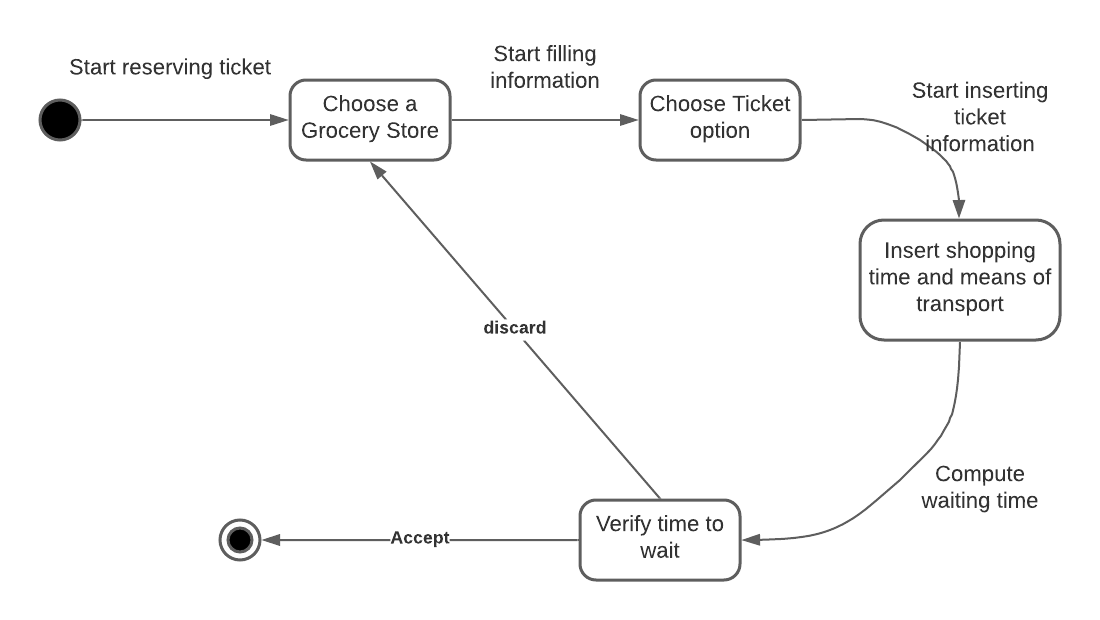
\includegraphics[height=0.3\textheight, scale=0.2, keepaspectratio]{img/Get_Ticket_diagram.png}
            \captionof{figure}{Getting ticket phase}
        \end{minipage}
    
    \item \textbf{Book a Visit}
    \begin{flushleft}
       A Customer correctly logged in, can see all the near store. After selecting one, he/she can book a visit. After selecting a store he/she have to specify the duration of the visit, select a time slot available and specify the categories of grocery that he/she want to buy in order to allow the System to calculate the best path in order to maximize social distancing. The time spent inside the grocery store is inferred and suggested using historical information.
       During the visit, the Customer can open the app and see the path suggested from the System.
    \end{flushleft}
    \begin{minipage}{\linewidth}
            \centering
          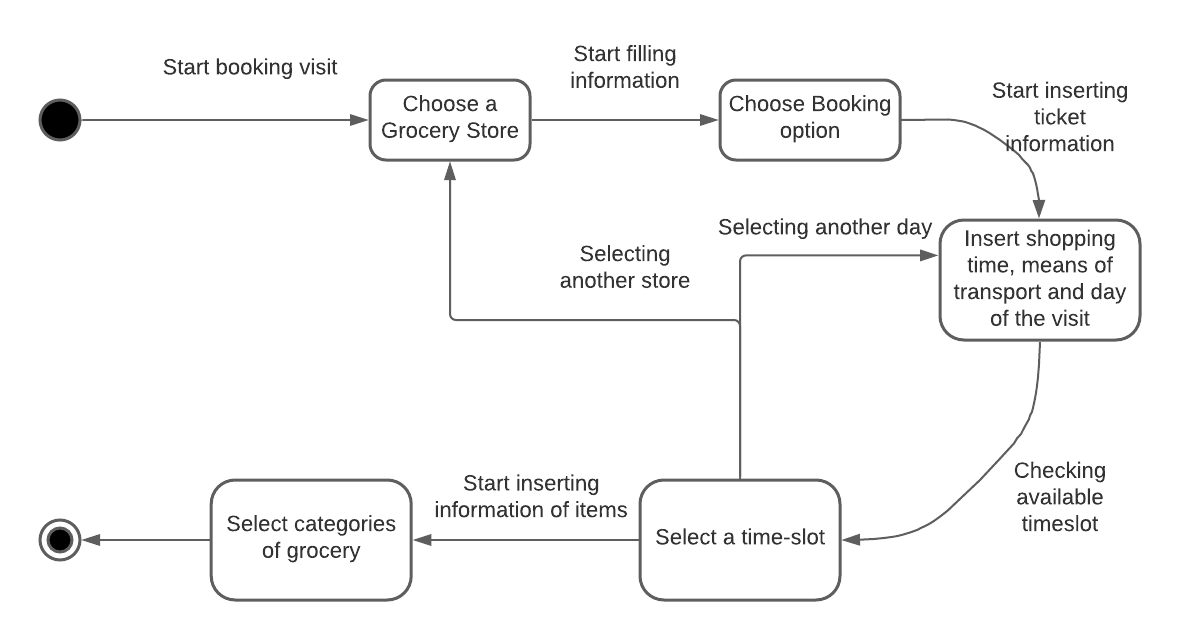
\includegraphics[height=0.3\textheight, scale=0.2, keepaspectratio]{img/Booking_diagram.png}
            \captionof{figure}{Booking a visit}
        \end{minipage}
        
    \item \textbf{Add a Store}
    \begin{flushleft}
        A Manager correctly logged in can add a new  Store.
        In order to create a Store a Manager should specify the name of the store, the address, the maximum number of people that can enter inside the store according to health directives, maximum number of people for each department of the store and opening hours. During this phase the Manager could specify other Managers of the store. After creation, he/she have to specify also credentials used by the System to verify that the store exists. At the end of this phase, a Manager upload a map of the stores, reporting information of the store such as walls, departments and category of grocery for each department.
    \end{flushleft}
    \item \textbf{Manage a Store}
    \begin{flushleft}
        A Manager correctly logged in can edit information of all his stores. He/she can edit the maximum number of people according to new health directives, modify the maximum number of people inside each department, map of the stores. He/she can also modify the managers, transfer ownership or delete a store from the System.
    \end{flushleft}
    \item \textbf{Perform a visit with ticket on App}
    \begin{flushleft}
        When is the turn of a Customer enqueque, before entering, he/she have to show his/her qr code to scanner machine in order to register the visit. \giovanni{Cosa accade durante la spesa se il tempo sfora quello richiesto?}.
        Once the Customer finish his shopping, during the payment, he/she scan one more time the qr code, in order to register the exit
    \end{flushleft}
    \item \textbf{Perform a visit with paper ticket}
     \begin{flushleft}
        When the Customer arrives to the grocery stores, get a ticket from the ticket machine. On the ticket is printed the entering time. Before entering the Customer have to show the qr code to scanner machine. Once the Customer finish his shopping, during the payment, he/she scan one more time the qr code, in order to register the exit
    \end{flushleft}
    \item \textbf{Perform a booked visit}
    \begin{flushleft}
        Before entering, the Customer scan his/her qr code. When he/she is inside, he can open the app and see the calculated path to follow in order to buy everything that he/she needs. Once the Customer finish his shopping, during the payment, he/she scan one more time the qr code, in order to register the exit
    \end{flushleft}
\end{enumerate}

\subsection{User Characteristics}

\subsection{Assumptions, Dependencies and Constraints}
\subsubsection{Assumptions}
\begin{enumerate}[label={DA.\arabic{*}}]
    \item \label{dom:fewPaperTickets} 
We assume that Paper Tickets will be few as in a situation of health emergency and social distancing people are invited to stay indoors.\lorenzo{FORSE NON TROPPO CHIARO}
    \item \label{dom:machineScanning}Each Store provides at least a Machine for Scanning.
    \item \label{dom:machinePaperTicket}Each Store provides at least as Machine for generating Paper Tickets.
    \item \label{dom:consumerAccessStore}The Consumers who enter a Store use a ticket, a paper ticket or a Visit and the vast majority of them scan their QR both at the entrance and at the exit.
\end{enumerate}
\section{Specific Requirements}
\label{specificRequirements}
\subsection{External Interface Requirements}
CL-up is a mobile based application, that can be also consulted using a web browser. Additional details regarding the hardware, software and communication interface requirements are described and shown below. There will also be some prototypes of User Interface for users who use mobile.

\subsubsection{User Interface}
%riga1
\begin{figure}[hbt]
\centering
\begin{subfigure}
	\centering
  	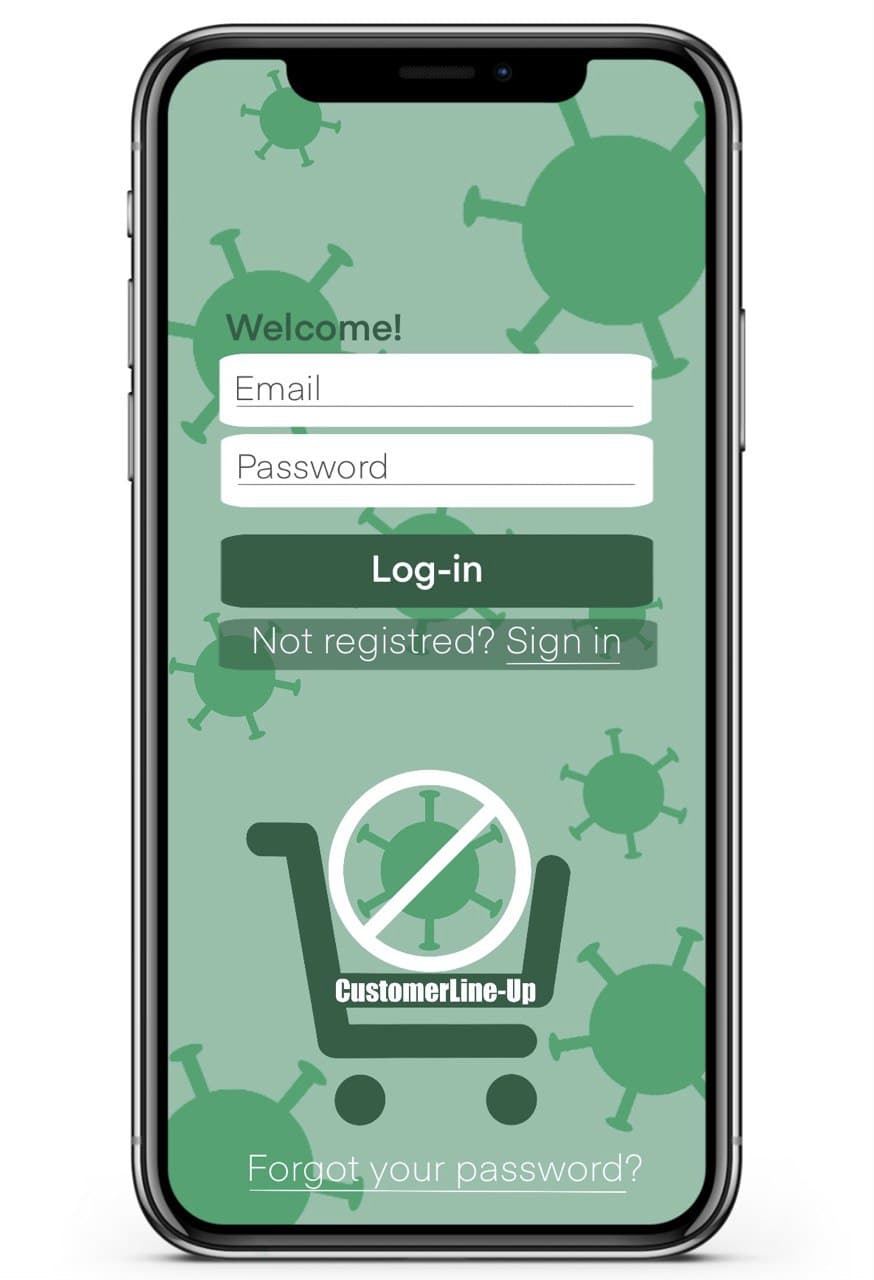
\includegraphics[height=0.3\textheight, scale=0.2, keepaspectratio]{img/GUI/login.jpg} 
 \end{subfigure}
 \begin{subfigure}
	\centering
  	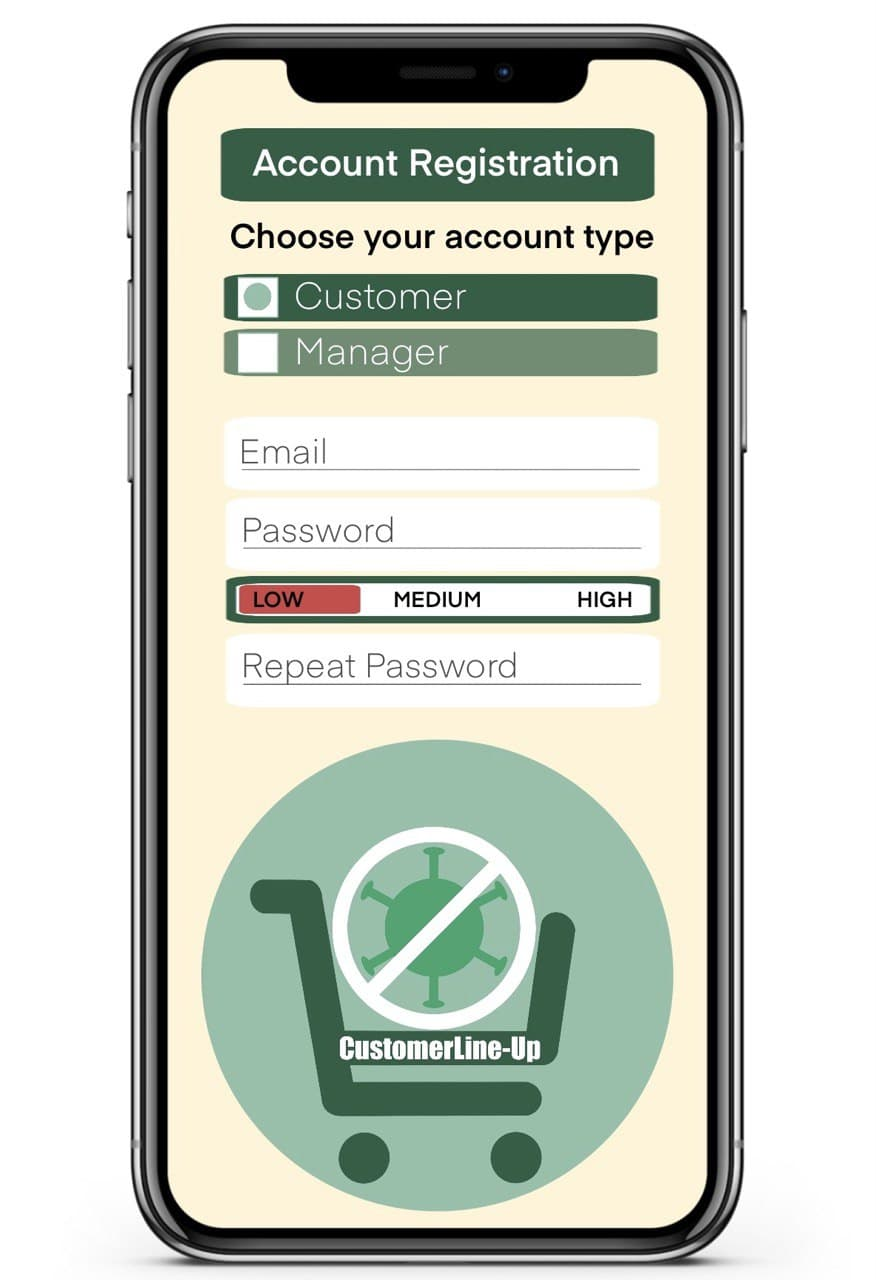
\includegraphics[height=0.3\textheight, scale=0.2, keepaspectratio]{img/GUI/registration.jpg}
 \end{subfigure}
	\caption{Guest login interface and signup interface.}
 	\label{entering}
\end{figure}
%riga2
\begin{figure}[h!]
\centering
\begin{subfigure}
	\centering
  	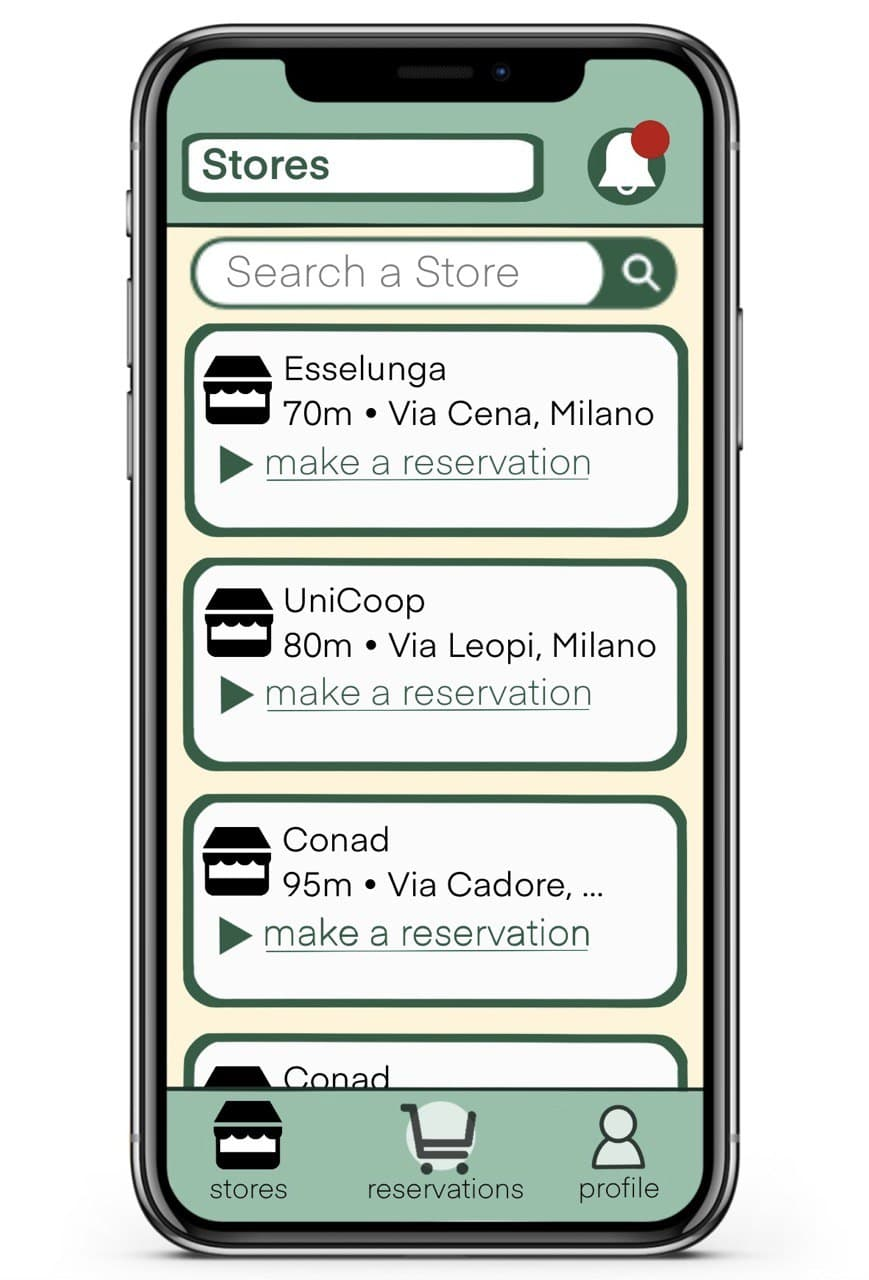
\includegraphics[height=0.3\textheight, scale=0.2, keepaspectratio]{img/GUI/stores_customer.jpg}
 \end{subfigure}
\begin{subfigure}
	\centering
  	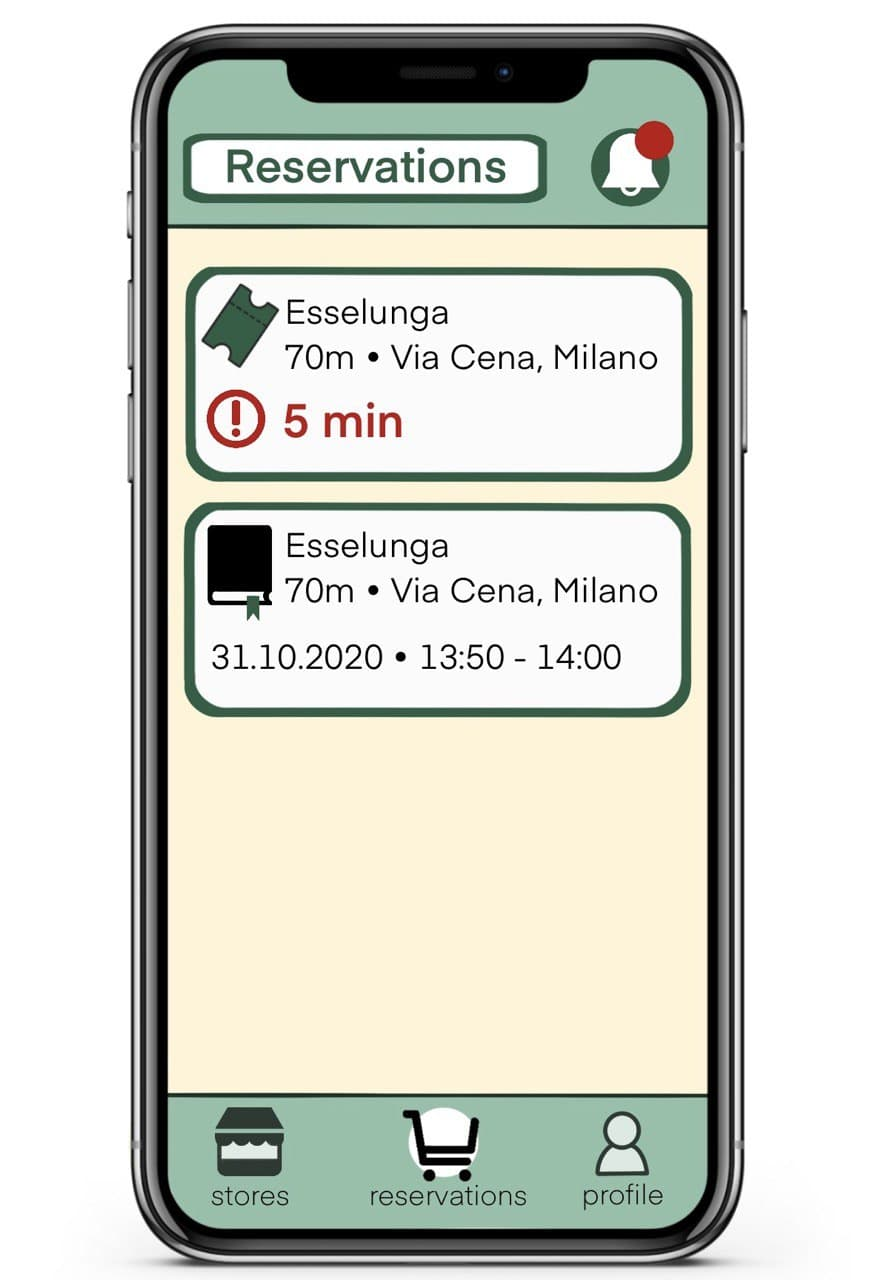
\includegraphics[height=0.3\textheight, scale=0.2, keepaspectratio]{img/GUI/main_customer.jpg} 
 \end{subfigure}
 \begin{subfigure}
	\centering
  	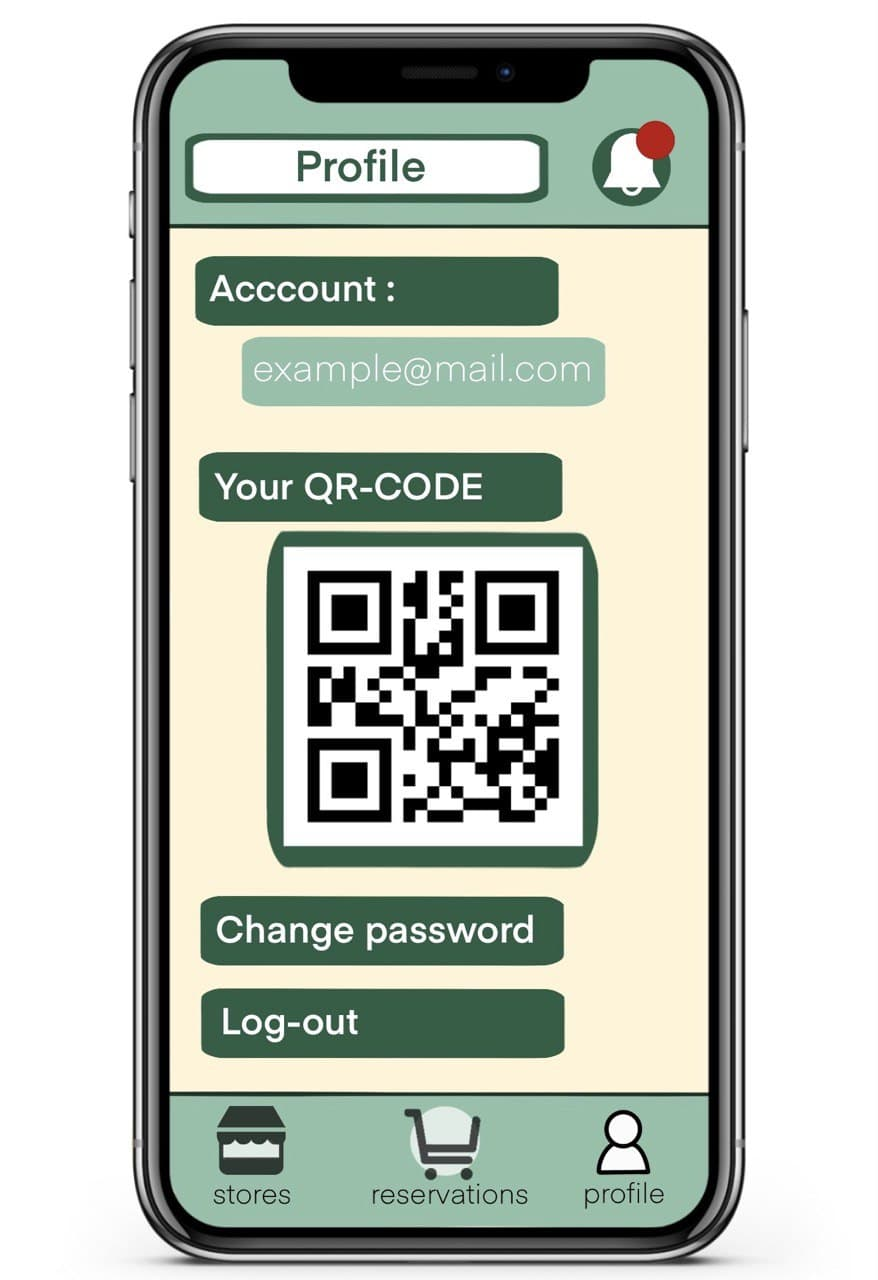
\includegraphics[height=0.3\textheight, scale=0.2, keepaspectratio]{img/GUI/profile_customer.jpg}
 \end{subfigure}
	\caption{Customers interfaces for list of Stores (for doing a Reservation), list of Reservations and profile.}
 	\label{customer screenshots}
\end{figure}
%riga3
\begin{figure}[h!]
\centering
\begin{subfigure}
	\centering
  	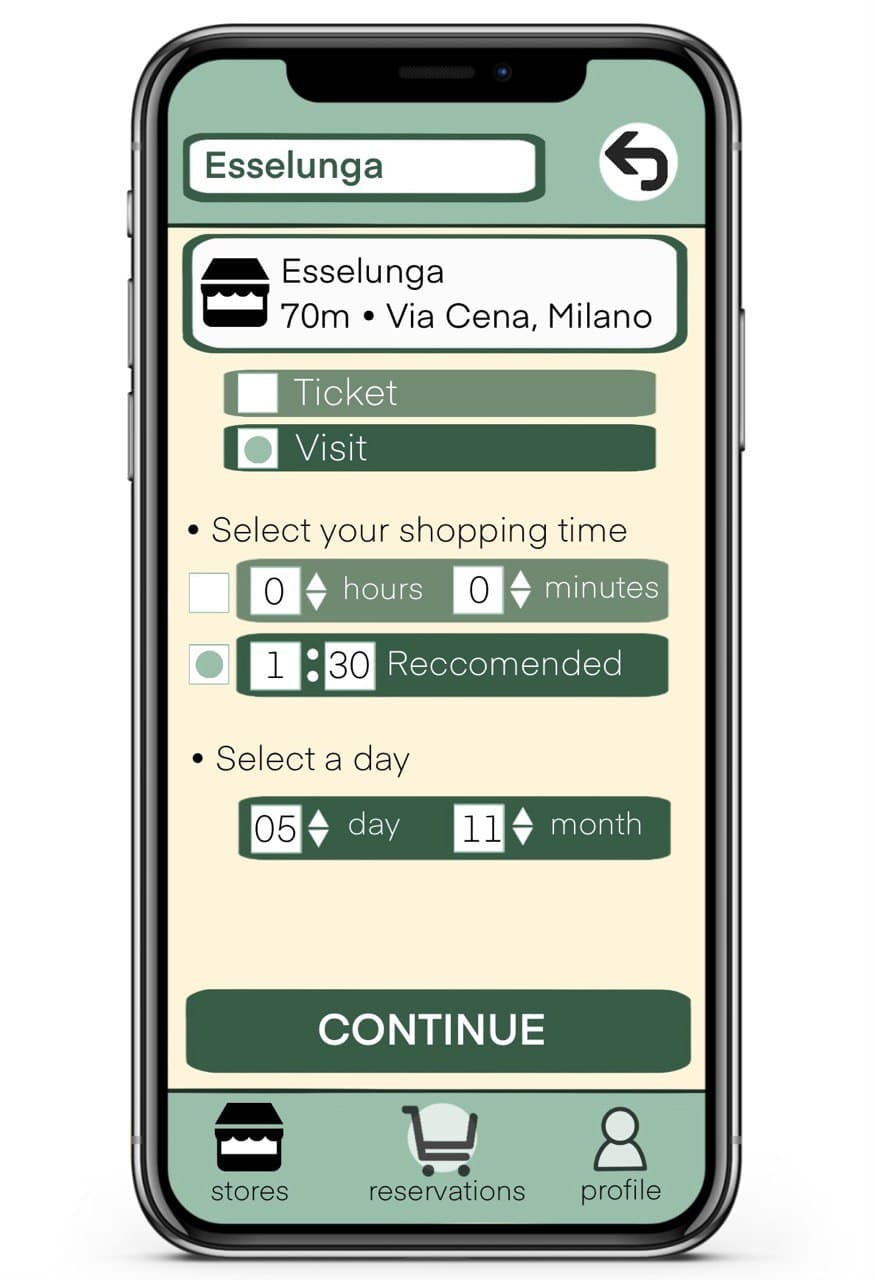
\includegraphics[height=0.3\textheight, scale=0.2, keepaspectratio]{img/GUI/book_visit_pt1.jpg}
 \end{subfigure}
\begin{subfigure}
	\centering
  	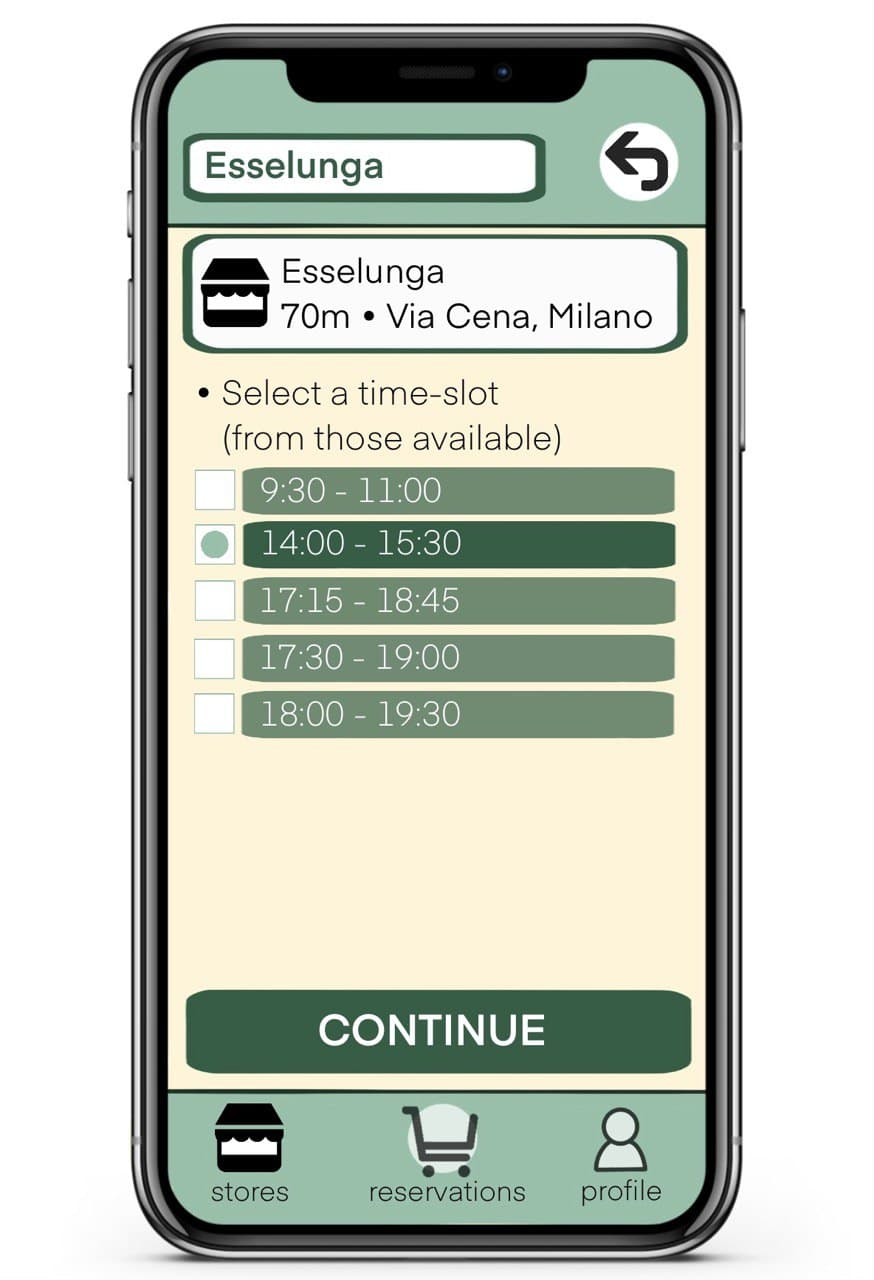
\includegraphics[height=0.3\textheight, scale=0.2, keepaspectratio]{img/GUI/book_visit_pt2.jpg} 
 \end{subfigure}
 \begin{subfigure}
	\centering
  	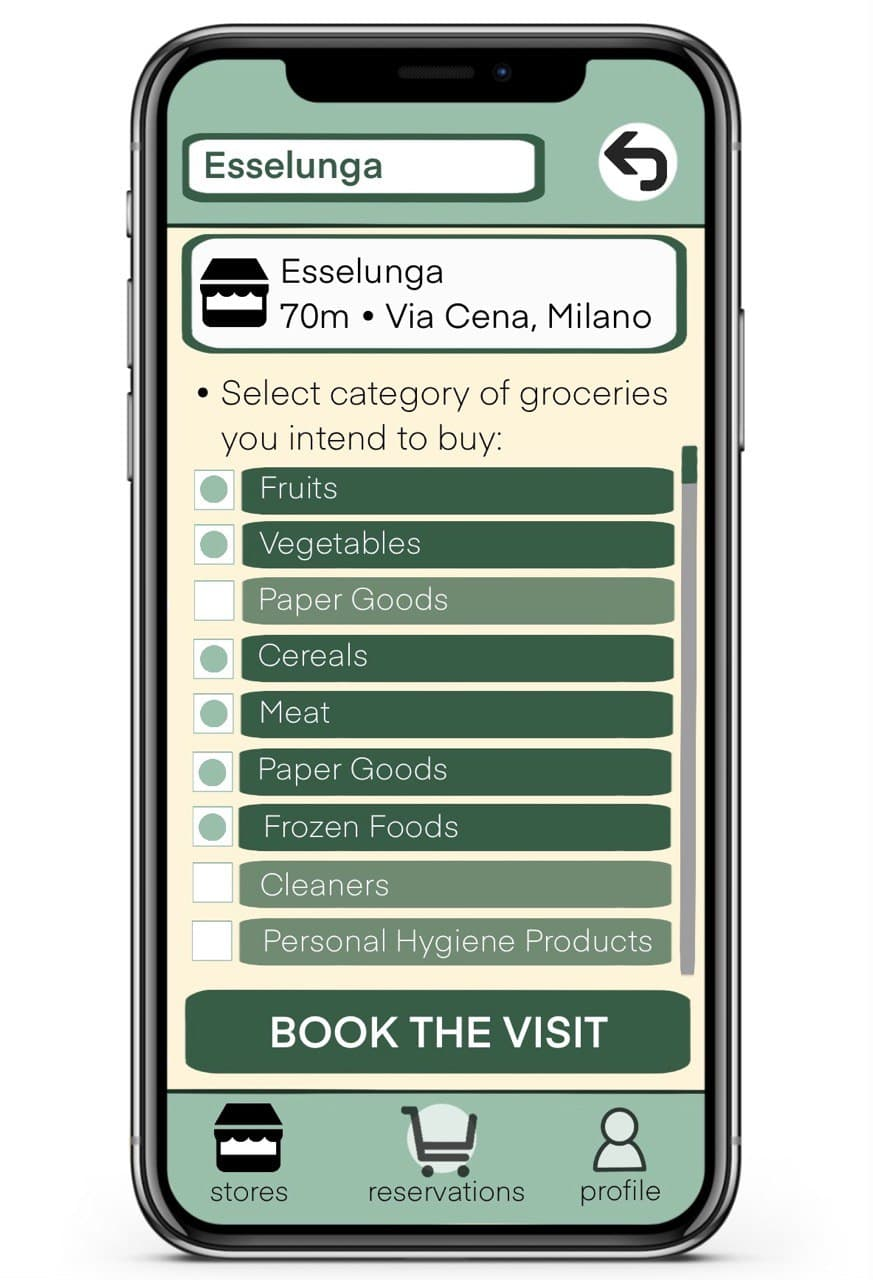
\includegraphics[height=0.3\textheight, scale=0.2, keepaspectratio]{img/GUI/book_visit_pt3.jpg}
 \end{subfigure}
	\caption{Customer interfaces for booking a Visit, once they have chosen the Store.}
 	\label{book a visit}
\end{figure}
%riga4
\begin{figure}[h!]
\centering
\begin{subfigure}
	\centering
  	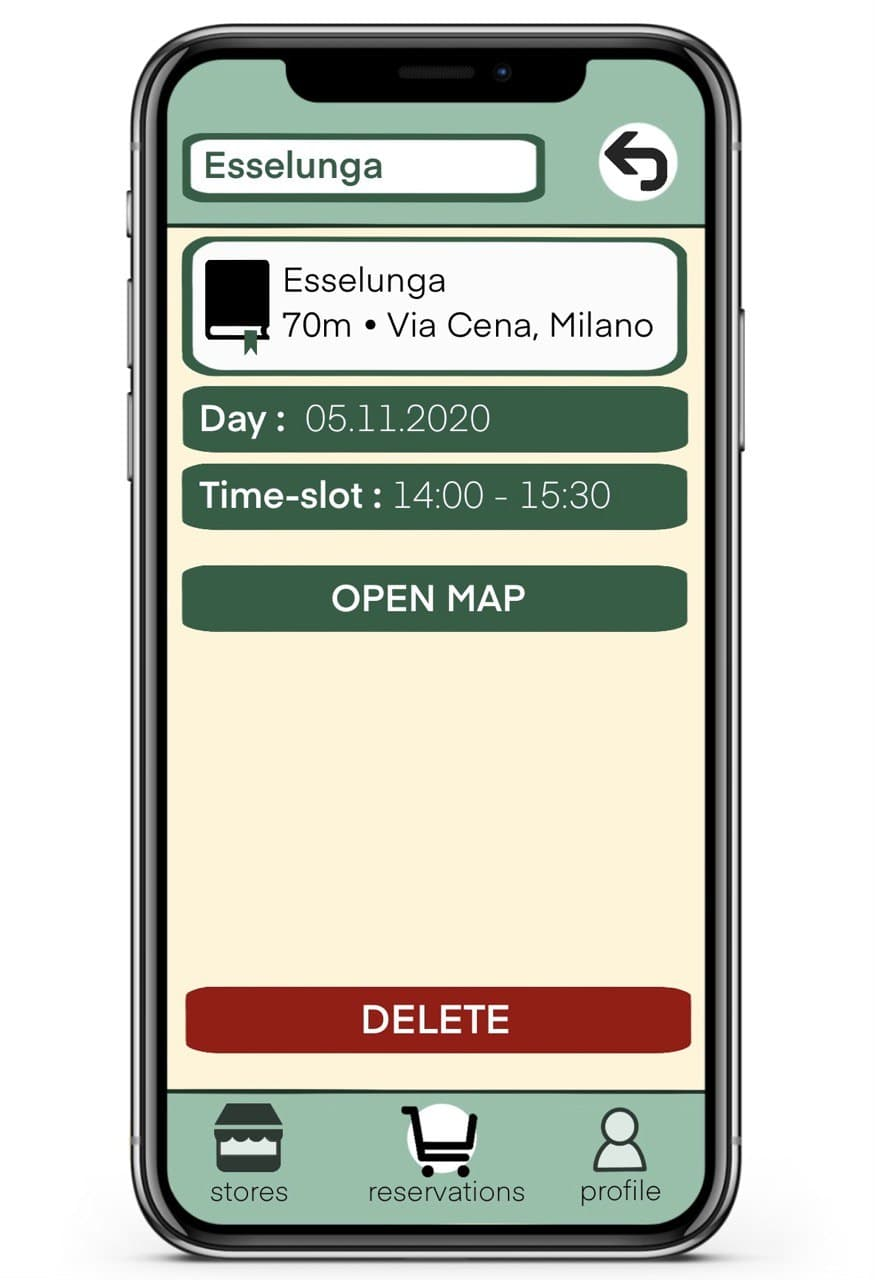
\includegraphics[height=0.3\textheight, scale=0.2, keepaspectratio]{img/GUI/visit_booked.jpg}
 \end{subfigure}
\begin{subfigure}
	\centering
  	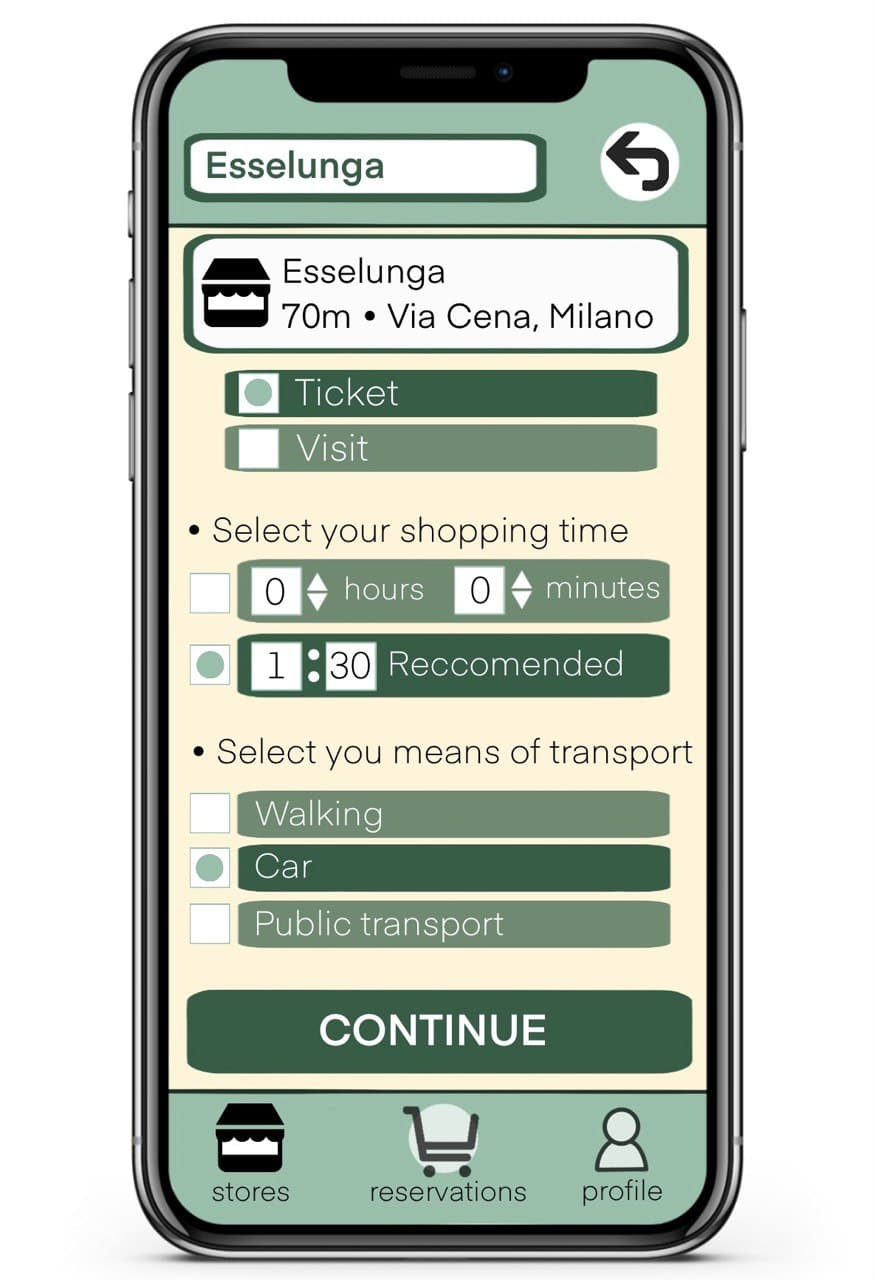
\includegraphics[height=0.3\textheight, scale=0.2, keepaspectratio]{img/GUI/get_ticket_pt1.jpg}
 \end{subfigure}
\begin{subfigure}
	\centering
  	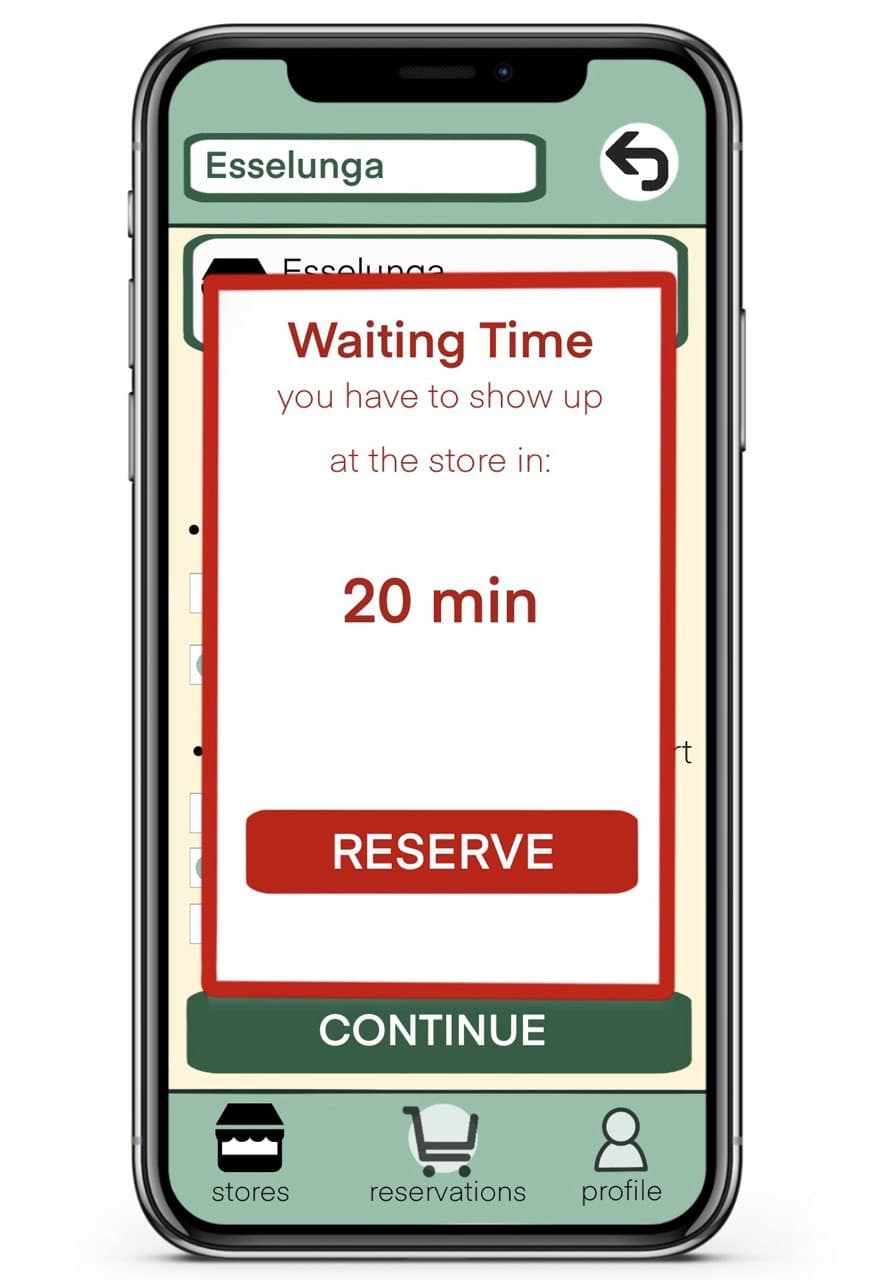
\includegraphics[height=0.3\textheight, scale=0.2, keepaspectratio]{img/GUI/get_ticket_pt2.jpg}
 \end{subfigure}
	\caption{Customer interfaces for booking a Virtual Ticket, once they have chosen the Store.}
 	\label{customer tickets}
\end{figure}
%riga 5
\begin{figure}[h!]
\centering
\begin{subfigure}
	\centering
  	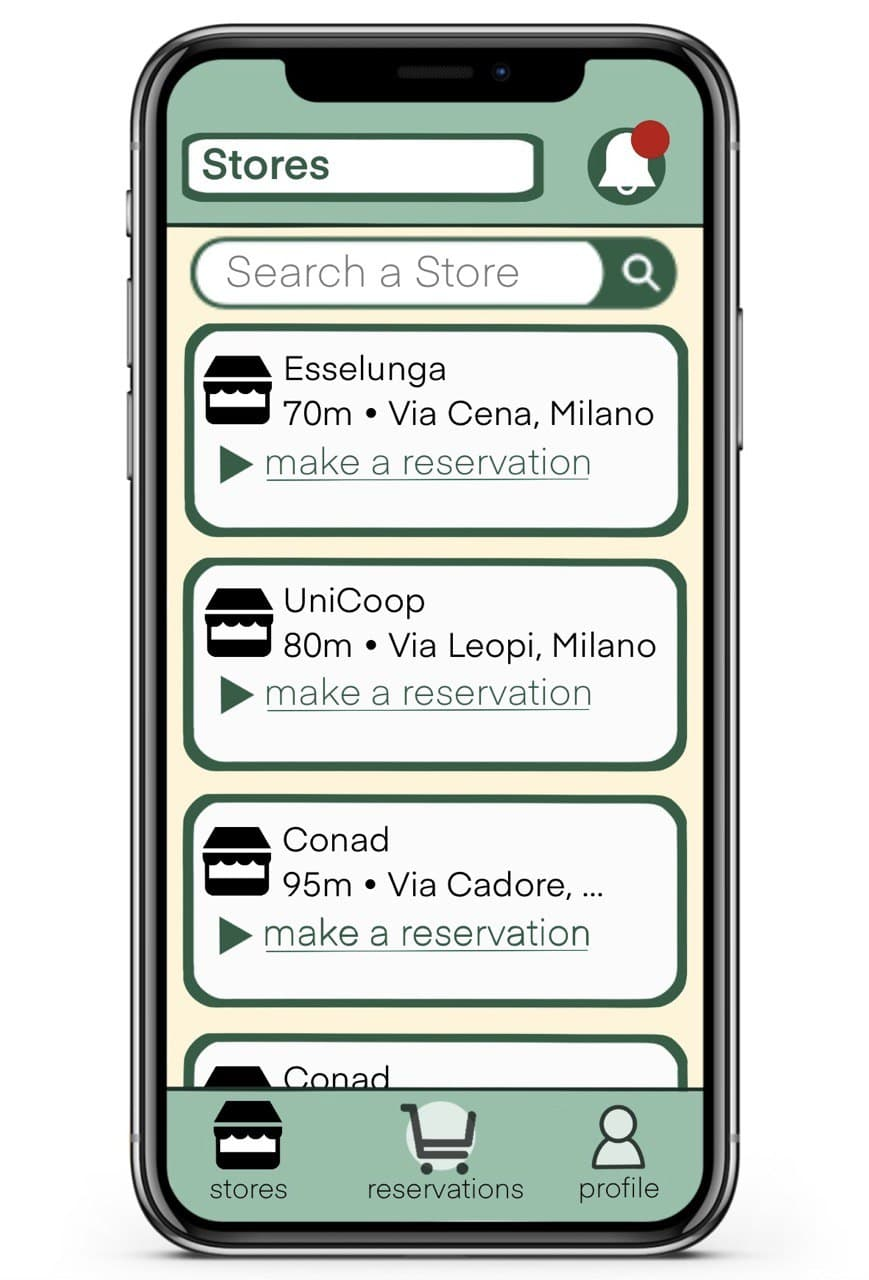
\includegraphics[height=0.3\textheight, scale=0.2, keepaspectratio]{img/GUI/stores_customer.jpg}
 \end{subfigure}
\begin{subfigure}
	\centering
  	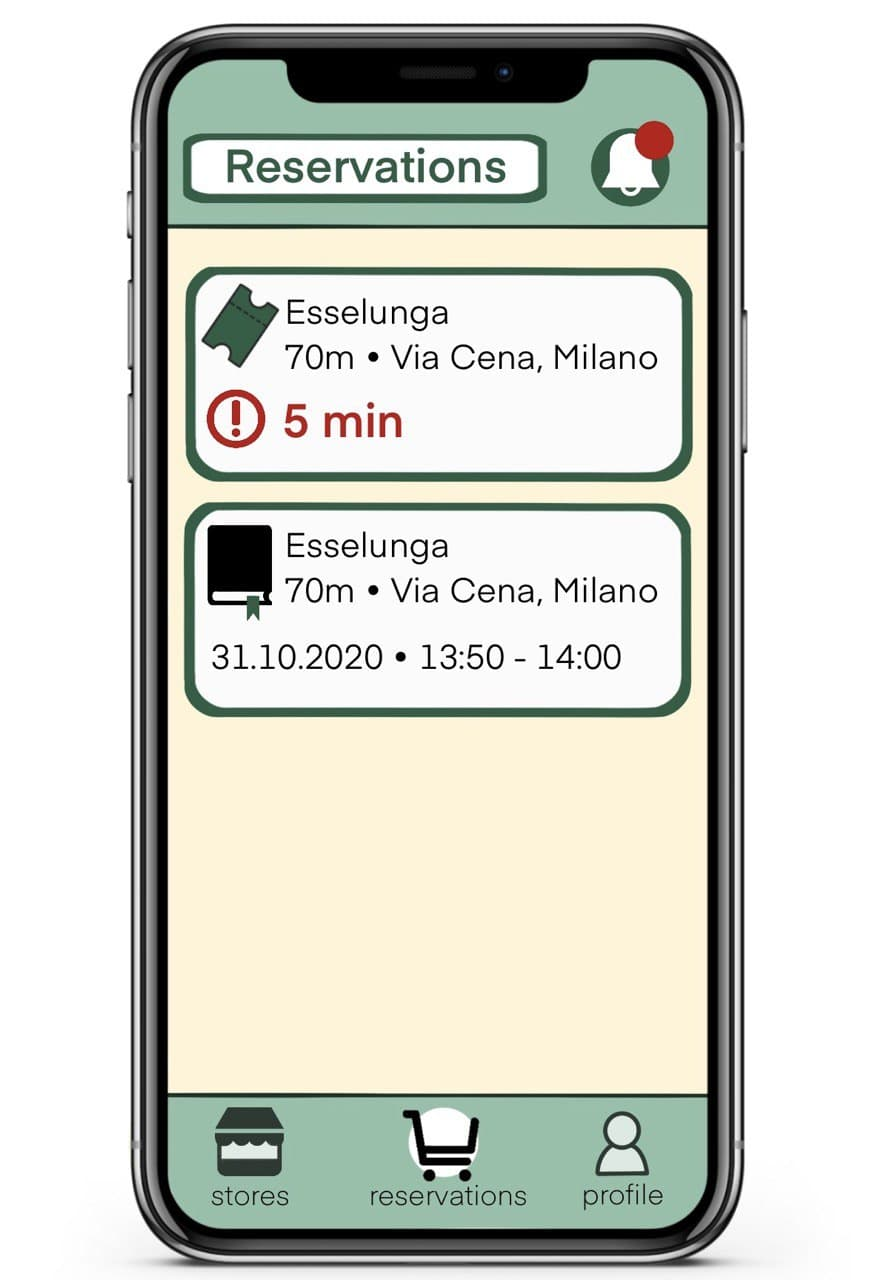
\includegraphics[height=0.3\textheight, scale=0.2, keepaspectratio]{img/GUI/main_customer.jpg} 
 \end{subfigure}
 \begin{subfigure}
	\centering
  	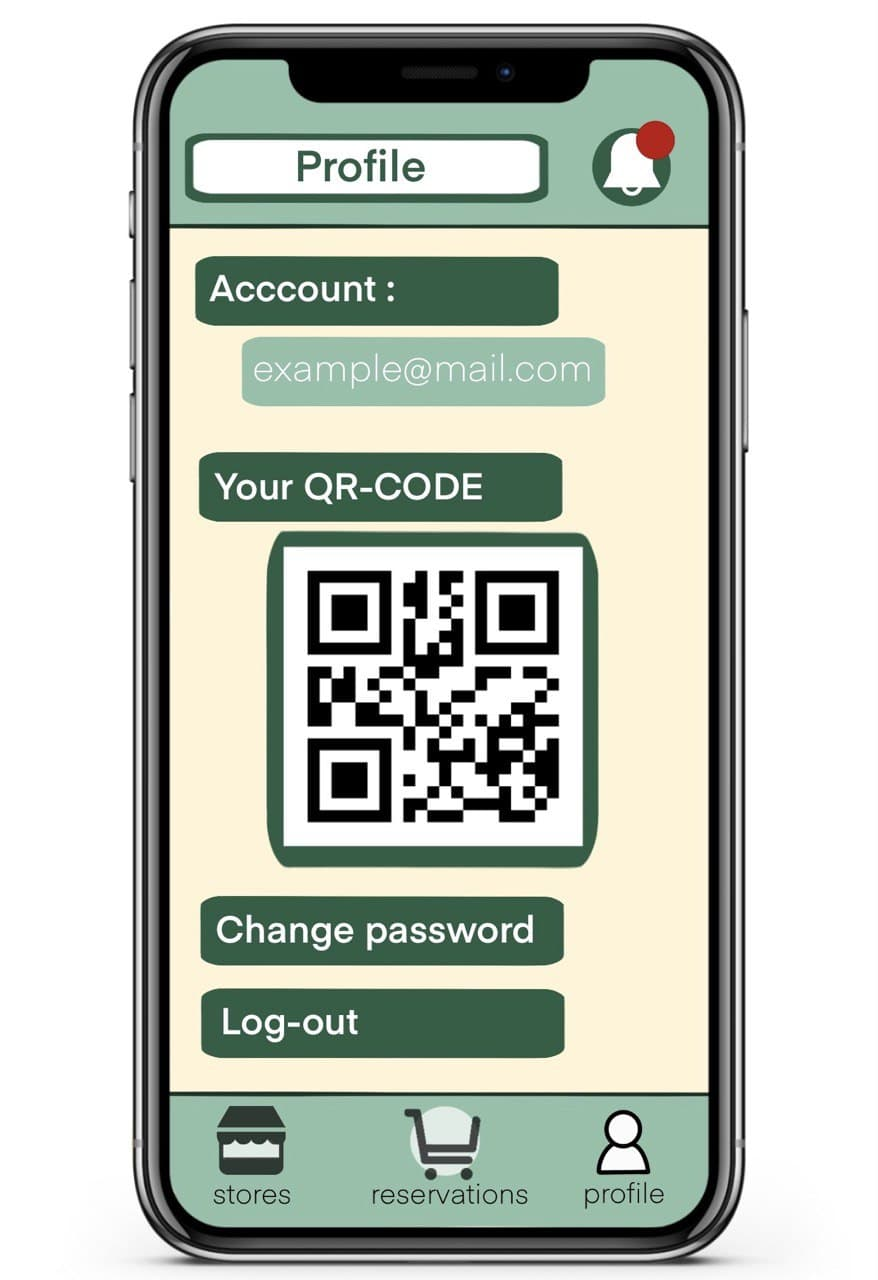
\includegraphics[height=0.3\textheight, scale=0.2, keepaspectratio]{img/GUI/profile_customer.jpg}
 \end{subfigure}
	\caption{Customers interfaces for list of Stores (for doing a Reservation), list of Reservations and profile.}
 	\label{customer screenshots}
\end{figure}
%riga3
\begin{figure}[h!]
\centering
\begin{subfigure}
	\centering
  	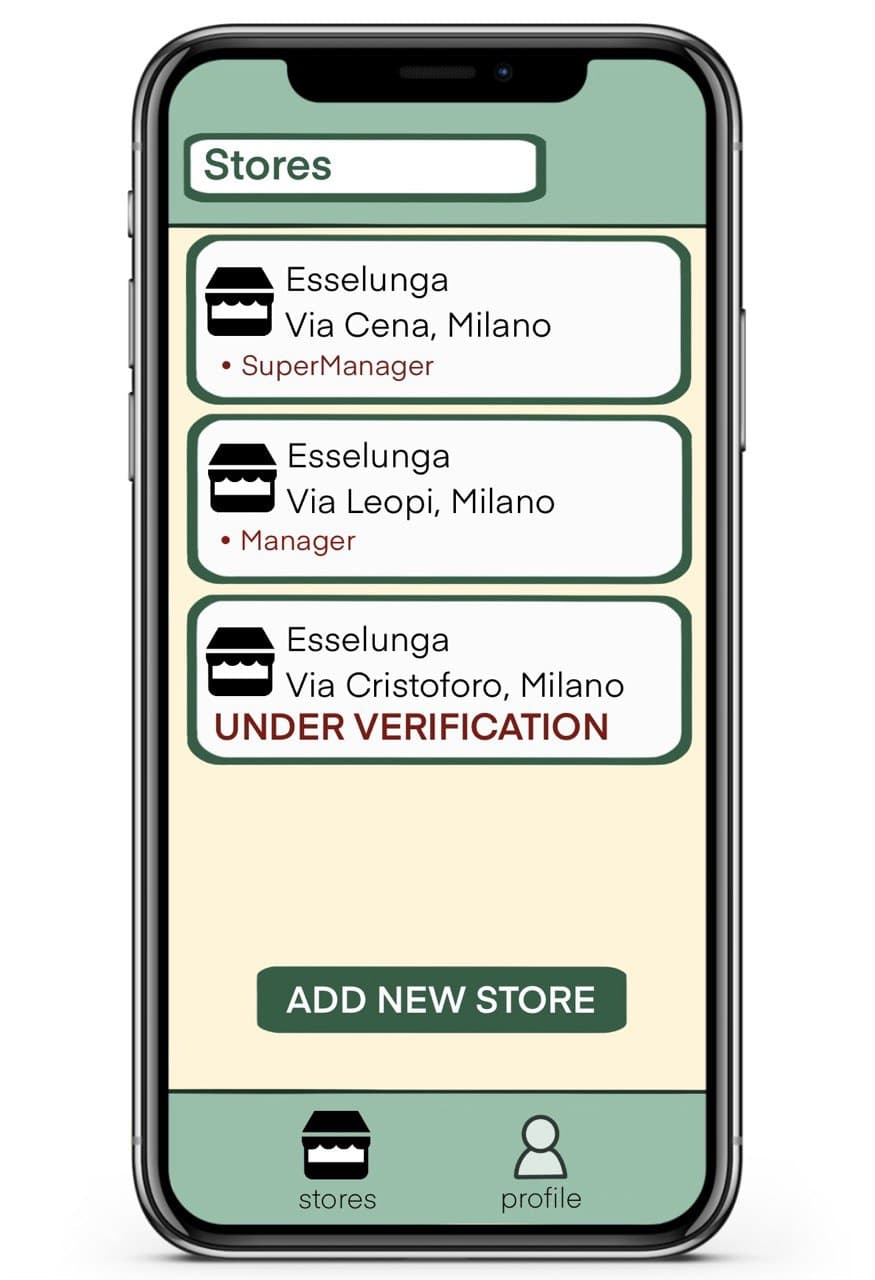
\includegraphics[height=0.3\textheight, scale=0.2, keepaspectratio]{img/GUI/main_manager.jpg}
 \end{subfigure}
\begin{subfigure}
	\centering
  	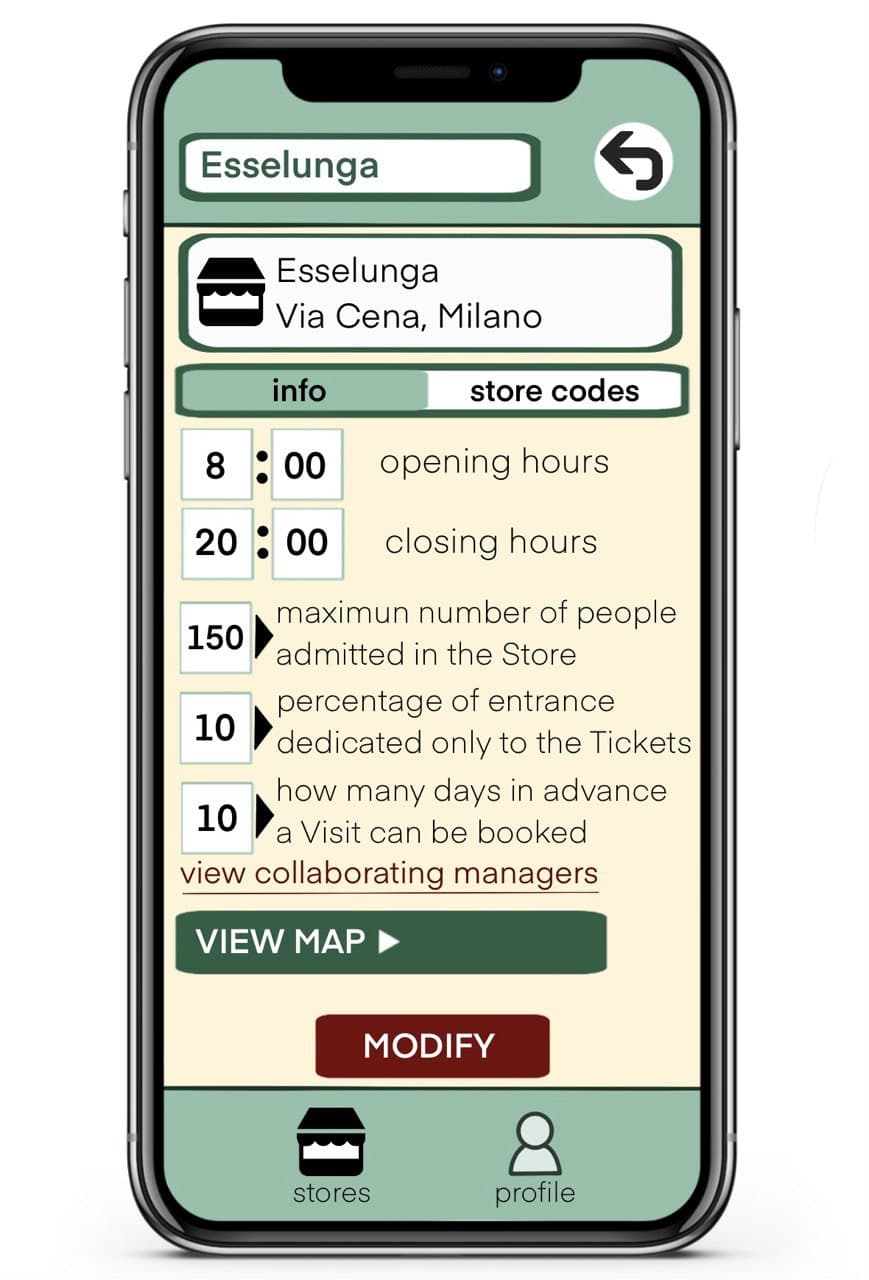
\includegraphics[height=0.3\textheight, scale=0.2, keepaspectratio]{img/GUI/manager_store_1.jpg}
 \end{subfigure}
 \begin{subfigure}
	\centering
  	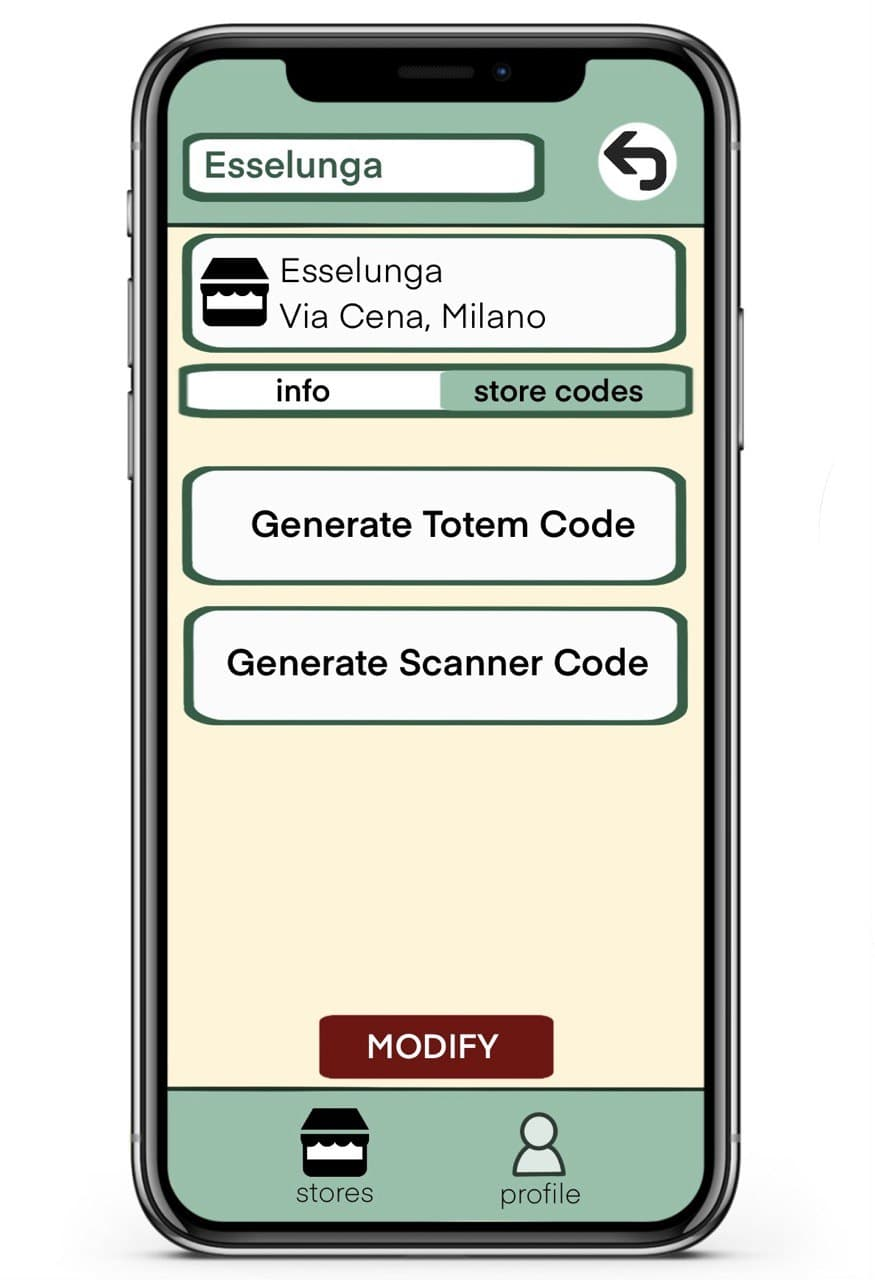
\includegraphics[height=0.3\textheight, scale=0.2, keepaspectratio]{img/GUI/manager_store_2.jpg}
 \end{subfigure}
	\caption{Manager interfaces to view the membership and owned Stores.}
 	\label{book a visit}
\end{figure}

\subsubsection{Hardware Interface}
The application is available for any type of mobile, having Internet access, a relatively recent browser, a GPS function, and enough storage space to accommodate the application itself.

\subsubsection{Software Interface}
\begin{enumerate}
\item[$\bullet$] Operating System: iOS, Android.
\item[$\bullet$] Web browser.
\item[$\bullet$] Web Server application.
\item[$\bullet$] DBMS.
\item[$\bullet$] Ticketing System: use third part services for GPS function. 
\item[$\bullet$] Mailing Service: APIs to send emails to the User
\item[$\bullet$] Queueing System: ??
\end{enumerate}

\subsubsection{Communication Interface}
The System runs over HTTPS protocol for the communication with application and notification system. The System also communicate with DBMS \giovanni{In qualche modo lo farà pure}.

\subsection{Functional Requirements}
\begin{enumerate}[align=left, label={R.\arabic{*}}]
    \item[\textbf{LOGIN \& REGISTER SERVICE}]
    \item \label{req:logOrReg} The User must be able to register or to log in if already registered.
    \item \label{req:credentialsCheck} Check if the User credentials are valid:
    \begin{enumerate}[label={-}]
        %\label{req:credentialsCheck:insert} 
        \item \label{req:credentialsCheck:email} Check that the email is in the right format.
        \item \label{req:credentialsCheck:uniqueness} Check that the email that the user is providing has not been used for previous registrations.
        \item \label{req:credentialsCheck:password}Check that the password is a Secure Password.
    \end{enumerate}
    \item \label{req:confirmRegistration}If the credentials are valid, the System sends a confirmation email, to let the user activate their account.
    \begin{enumerate}[label={-}]
        \item \label{req:confirmRegistration:timeout}If the User does not confirm their credentials within 24 hours, the account is removed and the credentials deleted.
    \end{enumerate}
    \item \label{req:login} Allow to log in using personal credentials:
    \begin{enumerate}[label={-}]
        \item \label{req:login:checkCred}Check if credentials are valid.
        \item \label{req:login:validCred} In case the email and password inserted are correct, allow the user to access all the functionalities available for the Type of User they are.
        \item \item \label{req:login:invalidCred} If the email and/or password inserted are wrong, the system must deny the access.
        \item If the username and/or password inserted are wrong, the system must notify the user. \lorenzo{Secondo me questo é da cancellare}
    \end{enumerate}
    \item \label{req:changeCredentials} Allow to change credentials, if the new credentials are in the right format.
    \item \label{req:changePassWithMail}Allow to change password if it has been forgotten, through the personal email.
    \item \label{req:provideQR} Provide to each Customer a unique QR code \lorenzo{which will be used as identifier in the enqueuing process}.
    \begin{enumerate}[label={-}]
        \item \label{req:provideQR:uniqueID} The QR code will be the identifier of the user within the System.
    \end{enumerate}
    \item \label{req:deleteAccount} Users must have the possibility to delete their accounts.
    
    \item[\textbf{TICKETING SERVICE}]
    \item \label{req:requestTicket} The Customer must be allowed to request a Ticket, specifying:
     \begin{enumerate}[label={-}]
        \item \label{req:requestTicket:store} The Store where he/she wants to shop.
        \item \label{req:requestTicket:duration}The duration of his/her shopping.
        \item \label{req:requestTicket:transport}The means of transport to get to the Store.
    \end{enumerate}
    \item \label{req:systemTicket}For Customers who are requesting a Ticket, the System should:
    \begin{enumerate}[label={-}]
        \item \label{req:systemTicket:verifyDist} Verify that their time distance from the Store is such that they can arrive in time for their turn.
        \item \label{req:systemTicket:addInQueue}Insert the Customer Ticket request in the queue in order to let the Customer arrive in time for his/her shopping.
        \item \label{req:systemTicket:waitingTime} Provide to the Customer the estimated waiting time before their turn.
        \item \label{req:systemTicket:notifForDepart} Notify Customers when they should depart from home in order to arrive in time for their turn.
        \item \label{req:systemTicket:reserveTimeout}The Customer, after receiving the request for confirming the ticket reservation, has some seconds to do it, otherwise the ticket is cancelled
    \end{enumerate}
    \item \label{req:numberTicketPerCust} Each Customer can request only one ticket. When they delete a request or they finish shopping in a Store and check out with the ticket or when the ticket expires, the Customer will be able to request another ticket.
    \label{req:codeUnique:ticketInfo}Every person on a Ticket can view the time in which they should enter the Store and the indicated duration of their shopping.
    
    \item[\textbf{BOOKING SERVICE}]
    \item \label{req:requestVisit}The Customer must be allowed to request a Visit, specifying:
    \begin{enumerate}[label={-}]
        \item \label{req:requestVisit:location}The Store where he/she wants to take a Visit.
        \item \label{req:requestVisit:date}The day of the Visit.
        \item \label{req:requestVisit:duration}The duration of his/her Visit.
        \item \label{req:requestVisit:timeslot}The time slot for the Visit.
        \item \label{req:requestVisit:categoriesToBuy}The Categories of Grocery he/her is going to buy.
    \end{enumerate}
    \item \label{req:statisticForDuration}For long time Customers, while booking a Visit, the System should infer, analyzing previous Visits of that Customer, the expected duration of the Visit. The Customer is free to use the suggestion or specify the time themselves the duration. \giovanni{Io sottolinerei che il tempo è consigliato, ma l'utente può cambiarlo} \lorenzo{FATTO}
    \item \label{req:sysProvideMap}The System should provide to the Customer a map of the Store.
    \begin{enumerate}[label={-}]
        \item \label{req:sysProvideMap:suggestPath}For Customers who have booked a Visit, the system should suggest to the Customer an optimal shopping path in order to buy everything they need, to minimize possible contacts between people inside the store and to shorten the time of the visit.
        \item \label{req:sysProvideMap:update} Each time the Customer views the map, the System checks if the current map is coherent with the Store information and updates it if not.
    \end{enumerate}
    \item \label{req:seeRequests}Allow Customers to consult their pending requests.
    \item \label{req:deleteTickOrVis}The Customer must be allowed to delete a Visit or a Ticket from his/her pending requests.
    \item \label{req:thirdPartyGPS}Use third party services to enable the localization of Customers and Stores. 
    \item \lorenzo{Notify Customers when they should depart from home in order to arrive in time for their Visit.} \yasmin{TO DELETE} \giovanni{LASCIALO} \lorenzo{TO DELETE} %\label{req:notifyCustomerToDepart}
    \item \label{req:notifyCustomerOpenSlots}Notify customers of available slots in a day-time range inferring information from their previous Visits.
    \item \label{req:visitPerDay} Each Customer can book up to three Visits in a single day.
    
    \item \label{req:expiredTickOrVis} If a Visit/ticket is expired, or it has served its purpose, or it has been deleted, it will be removed and will not be visible to the Customer anymore 
    
    \item[\textbf{STORE MANAGEMENT SERVICE}]
    \item \label{req:man:createStore}Allow Managers to create Stores, becoming the Owner of the Store.
    \begin{enumerate}[label={-}]
        \item \label{req:man:createStore:nameAndLoc}Allow to specify name of the Store and his address
         \item \label{req:man:createStore:maxPeople}Allow Managers to specify maximum number of people who can enter the Store.
        \item \label{req:man:createStore:maxPeoplePerDep}Allow Managers to specify maximum number of people for each Department of the Store.
        \item \label{req:man:createStore:openingHours}Allow Managers to specify Store opening hours.
        \item \label{req:man:createStore:daysToBook}Allow managers to specify how many days in advance a Visit can be booked
        \item \label{req:man:createStore:percentageTicket} Allow Managers to specify the percentage of Capacity of the Store reserved exclusively for Ticket's reservations.
    \end{enumerate}
    \item \label{req:man:deleteStore}Allow Owner to delete their Stores.
    \item \label{req:man:verifyOwnerCred}Verify the Store creation, acquiring specific credentials that can be used to verify the validity of the Store and of the Manager. \lorenzo{(During the creation of a Store ask for an associated PEC)}
    \item \label{req:man:updateStoreInfo}Allow the Owner and Managers to edit the store:
    \begin{enumerate}[label={-}]
         \item \label{req:man:updateStoreInfo:maxPeople}Allow Managers to edit maximum number of people who can enter the Store.
        \item \label{req:man:updateStoreInfo:maxPeoplePerDep}Allow Managers to edit maximum number of people for each Department of the Store.
        \item \label{req:man:updateStoreInfo:openingHours}Allow Managers to edit Store opening hours.
         \item \label{req:man:updateStoreInfo:addMan}Allow Owner to add other Managers to their Store(s).
        \item \label{req:man:updateStoreInfo:removeMan}Allow Owner to remove Managers from their Store(s).
        \item \label{req:man:updateStoreInfo:handOwnership}Allow Owner to hand over the ownership of the Store to one of its Managers.
        \item \label{req:man:updateStoreInfo:daysToBook}Allow managers to edit how many days in advance a Visit can be booked.
    \end{enumerate}
    
        \item \label{req:man:whenToUpdate}All the information about the Store can be updated by their Managers at anytime
    \begin{enumerate}[label={-}]
        \item \label{req:man:whenToUpdate:whenEffective}If the updates change opening hours or the maximum number of people in the store or how many days in advance a Visit can be booked, the Manager will have two options: make the updates effective within 24 hours, losing booked Visits which are not valid anymore, or make the updates effective within the current amount of how many days in advance a Visit can be booked without taking a chance on losing booked Visits.
        \item \label{req:man:whenToUpdate:lostVisits} If some Visits are cancelled, the System notify the Customers involved.
    \end{enumerate}
    
    \item \label{req:man:uploadMap}Allow Managers to upload a map of their Stores:
    \begin{enumerate}[label={-}]
        \item \label{req:man:uploadMap:GUI}Provide a GUI to specify the structure of the Store to the System (walls, Departments, category of grocery for each Department)
        \item \label{req:man:uploadMap:specCategories}Allow the Managers to specify Categories of groceries for each Department.
        \item \label{req:man:uploadMap:specInCategories}Allow Managers to specify groceries and brands for each Department. \lorenzo{!!! let's talk about the difference between department and categories of grocery.}
    \end{enumerate}
    
    \item \label{req:scannerApp}Provide a specific \textbf{Scanner App} to scan the QR codes of the Consumers and to interact with the queuing mechanism.
    \begin{enumerate}[label={-}]
        \item \label{req:scannerApp:response} Once a Scanner scan a QR code it can visualize one of this messages: if the Consumer of that QR code can enter the Store, or if he is still in the queue (it's not his turn yet), or if his reservation has been deleted (because of Queue Scaling Process or because he never reserved anything).
        \item \label{req:scannerApp:createCode} The Managers of a Store can create a unique identifier linked to the store to input it to Scanner APP to enable its functions.
    \end{enumerate}
    
    \item \label{req:paperTicketApp}Provide a specific \textbf{Paper Tickets App} to generate paper tickets in the store and to interact with the queuing mechanism.
    \begin{enumerate}[label={-}]
        \item \label{req:paperTicketApp:func}The Paper Ticket app will allow every person to get a Paper Ticket directly from the Store.
        \item \label{req:paperTicketApp:funcPaperTick}In the Paper Tickets there will be specified the same information provided with the online Ticket and it will work the same way. The associated QR code will be automatically generated by the Paper Ticket app, and it will be different from the QR codes of each Customer (i.e. User registered in the main app).
        \item \label{req:paperTicketApp:createCode}The Managers of a Store can create a unique identifier linked to the store to input it to the Paper Ticket app to enable its functions.
    \end{enumerate}
    
    
    \item \label{req:queueUnique}Each Store has one and only one queue.
    \begin{enumerate}[label={-}]
        %\item \label{req:codeUnique:queueVector} The queue for each day is as long as the number of minutes the Store is open divided by 5, ie a Temporal Quantum.
        %\item \label{req:codeUnique:vectorOfVectors} Every Temporal Quantum of the queue contains as many elements as the capacity of the Store.
        %\item \label{req:codeUnique:queueReservations} Every time a Consumer makes a Reservation, it is occupied an element in every Temporal Quantum he needs, that is the Duration of Shopping divided by 5, if and only if the System can find sequential empty spaces (ie an empty space in different subsequent Temporal Quantums of the queue) within the queue. The spaces occupied in each Temporal Quantum will be the first available in that Temporal Quantum.
        \item \label{req:codeUnique:queueReservations}Every time a Consumer makes a Reservation, some spaces on the queue are searched and reserved, in order to let him have enough time for the duration of his shopping.
        \item \label{req:codeUnique:visitsAndQueue} Consumers who have booked a Visit will be inserted in the same queue of the ones who have got a (paper or virtual) Ticket, but they will have higher priority.
        \item \label{req:codeUnique:ticketsAndQueue} Consumers with a Paper Ticket have a higher priority than the ones with Virtual Tickets.
        \item Only the Customers will have the entering time updated in real time. %The time of the Visits must be updated as a last resort.
        \item \label{req:codeUnique:invalidateLate} If the Consumer will not show up in time for their Reservation, %that is if the store Scanner does not receive the scan of the QR Code relating to the Consumer before the ending of the first Temporal Quantum of their Reservation,
        their Reservation will be considered invalid and it will be cancelled.
        \item \label{req:codeUnique:exeedDuration} A Consumer which does not go out of the shop within the duration declared will activate the Queue Scaling Process and the duration of his/her visit will be extended.% (for clarifications on the Queue Scaling Process, go to chapter ...)
        \item \label{req:codeUnique:queueScaling} The scaling of Consumers in the queue has to be done in such a way that Consumers can be scaled only forward and not backwards. %(for clarifications on the Queue Scaling Process, go to chapter ...)
        \item \label{req:codeUnique:scalingExceed} During the Queue Scaling Process, any scaling that causes a Reservation to exceed the closing hours will lead to the cancellation of the Reservation.
        \item \label{req:codeUnique:scalingOverlap} During the Queue Scaling Process, any scaling that causes a Virtual Ticket or Visit to overlap with another Virtual Ticket or Visit of the same Costumer (also for different Stores), there will be a cancellation of one of the Reservations. \yasmin{dovrei specificare con quale priorità} 
        \item \label{req:codeUnique:queueNotifications} Every time a Reservation of a Customer is cancelled, the Customer must be notified.
        \item \label{req:codeUnique:queueLast30} The last 30 minutes in which a Store is open cannot be booked by any type of Reservation, so that they can be exploited within the Queue Scaling Process, in order to eventually have to eliminate a smaller number of Reservations.
        %\item \label{req:codeUnique:queueReset} When the Store closes (each day) the queue resets it states, keeping only the booked Visits for the next days.
        \item \label{req:codeUnique:reset} The queue should be made in such a way that after the closing hours of a Store, it delete every old Reservations, that is every Reservation made for that day. In this way just future booked Visits are preserved.
        \item \label{moreOpeningHours} The queue has to be made in such a way that, also if there are more opening and closing hours of a Store in a single day,% the number of intermediate Temporal Quantums (in which the Store is closed) must be blocked
        closing hours can't be booked and can't be scaling in between.% This means that those blocked Temporal Quantums cannot be booked and it is not possible to make scales that go beyond them.
        
        %\item \lorenzo{DA METTERE NELLE DEFINIZIONI O SPECIFICHE}Queue Scaling: the system checks if the number of people in the Store is less than or equal of the capacity of the store in each period of time (this will be chosen during the implementation process). If not, the system will change the entrance time of some customers to validate the aforementioned constraint. The order of the people with online tickets and booked visits in the queue will be preserved . The time of entrance can be only delayed. The time of entrance of people with paper ticket is frozen (cannot be changed).
    \end{enumerate}

    \item \label{req:inferringSuggestions}Suggestions are based on the habits of the Customers, inferred by the Data Analytics Manager. In a first period will be suggested Stores which are available and geographically close to the Customer (within 1 km). 
\end{enumerate}

\label{uc:gToReDMatrix}
\begin{center}
{\textbf{Goal to requirements and domain assumptions Matrix}}
\end{center}

\begin{tabularx}{\linewidth}{| p{20mm} | p{50mm} | p{50mm} |}

    % UC GOAL REQ DOMAIN
     \hline
	GOALS & REQUIREMENTS & DOMAIN ASSUMPTIONS \\
	\hline 
	\ref{goal:auth} & \ref{req:logOrReg}, \ref{req:credentialsCheck}, \ref{req:confirmRegistration}, \ref{req:login}, \ref{req:changeCredentials}, \ref{req:changePassWithMail}, \ref{req:deleteAccount}, \ref{req:expiredTickOrVis}, \ref{req:man:verifyOwnerCred} & --- \\
	
	\hline
	\ref{goal:influx} & \ref{req:provideQR} & \ref{dom:machineScanning}, \ref{dom:machinePaperTicket}, \ref{dom:consumerAccessStore}, \ref{req:man:createStore}, \ref{req:man:deleteStore}, \ref{req:man:updateStoreInfo}, \ref{req:scannerApp}, \ref{req:paperTicketApp}, \ref{req:queueUnique} \\
	
	 \hline 
	\ref{goal:effectiveQueue} & \ref{req:provideQR}, \ref{req:thirdPartyGPS}, \ref{req:man:updateStoreInfo}, \ref{req:man:whenToUpdate}, \ref{req:man:uploadMap}, \ref{req:queueUnique} & \ref{dom:fewPaperTickets}, \ref{dom:machineScanning}, \ref{dom:machinePaperTicket}, \ref{dom:consumerAccessStore} \\
	
	\hline
	\ref{goal:enqueue} & \ref{req:requestTicket}, \ref{req:systemTicket}, \ref{req:numberTicketPerCust}, \ref{req:codeUnique:ticketInfo}, \ref{req:deleteTickOrVis}, \ref{req:thirdPartyGPS} & ---  \\

	\hline
	
	\ref{goal:visit} & \ref{req:requestVisit}, \ref{req:statisticForDuration}, \ref{req:sysProvideMap}, \ref{req:seeRequests}, \ref{req:deleteTickOrVis}, \ref{req:thirdPartyGPS}, \ref{req:notifyCustomerOpenSlots}, \ref{req:visitPerDay}, \ref{req:inferringSuggestions}  & ---  \\

	\hline
	
\end{tabularx}


\subsubsection{Use Cases}
\begin{enumerate}[labelindent=20pt, label={UC.\arabic*}, itemindent=1em,leftmargin=!]
    % both customer and manager
    \item Registration \label{uc:registration}
    \item Login \label{uc:login}
    \item Update Credentials \label{uc:updateCredentials}
    \item Lost Password \label{uc:lostPassword}
    % customer
    \item Get Ticket \label{uc:getTicket}
    \item Book Visit \label{uc:getVisit}
    \item Access Store \label{uc:accessStore}
    \begin{enumerate}[label={-}]
        \item Using Ticket
        \item Using Visit
    \end{enumerate}
    \item Delete Ticket/Visit \label{uc:deleteBooked}
    % manager
    \item Create Store \label{uc:createStore}
    \item Activate Scanner \label{uc:useScanner}
    \item Activate Paper-ticket machine \label{uc:usePaper}
    \item Update Store info \label{uc:updateStoreInfo}
\end{enumerate}
\label{uc:traceabilityMatrix}
\begin{center}
{\textbf{Traceability Matrix}}
\end{center}

\begin{tabularx}{\linewidth}{| p{20mm} | p{20mm} | p{30mm} | p{50mm} |}

    % UC GOAL REQ DOMAIN
     \hline
	USE CASES & GOALS & REQUIREMENTS & DOMAIN ASSUMPTIONS \\
	 \hline
	\ref{uc:registration} & \giovanni{\ref{goal:auth}} & \ref{req:logOrReg}, \ref{req:credentialsCheck}, \ref{req:confirmRegistration}, \ref{req:provideQR}  & ---\\
	
	 \hline
	\ref{uc:login} & \ref{goal:auth} & \ref{req:logOrReg}, \ref{req:credentialsCheck}, \ref{req:login} & --- \\
	
	\hline
	\ref{uc:updateCredentials} & \ref{goal:auth} & \ref{req:changeCredentials} & --- \\

	\hline
	\ref{uc:lostPassword} & \ref{goal:auth} & \ref{req:changePassWithMail} & --- \\
	
	\hline
	% \hline
	% \textbf{Achieved Goals} & {}\\
	\ref{uc:getTicket} & \ref{goal:influx}, \ref{goal:effectiveQueue}, \ref{goal:enqueue} & \ref{req:requestTicket}, \ref{req:systemTicket}, \ref{req:numberTicketPerCust} & --- \\
	\hline
	
	\ref{uc:getVisit} & \ref{goal:influx}, \ref{goal:effectiveQueue}, \ref{goal:visit} & \ref{req:requestVisit}, \ref{req:visitPerDay}, \ref{req:statisticForDuration}, \ref{req:visitPerDay} & --- \\
	\hline
	
	\ref{uc:accessStore} & \ref{goal:influx}, \ref{goal:effectiveQueue}, \ref{goal:enqueue}, \ref{goal:visit} & \ref{req:sysProvideMap}, \ref{req:thirdPartyGPS}, \ref{req:inferringSuggestions} & \ref{dom:machineScanning}, \ref{dom:machinePaperTicket}, \ref{dom:consumerAccessStore}, \ref{dom:consumerAccessStore} \\
	\hline
	
	\ref{uc:deleteBooked} & --- & \ref{req:deleteTickOrVis}, \ref{req:expiredTickOrVis} & --- \\
    \hline
    
    \ref{uc:createStore} & --- & \ref{req:man:createStore}, \ref{req:man:verifyOwnerCred} & --- \\
    \hline
    
    \ref{uc:useScanner} & \ref{goal:influx}, \ref{goal:enqueue} & \ref{req:scannerApp} & \ref{dom:machineScanning}\\
    \hline
    
    \ref{uc:usePaper} & \ref{goal:influx}, \ref{goal:enqueue} & \ref{req:paperTicketApp} & \ref{dom:machinePaperTicket}\\
    \hline
    
    \ref{uc:updateStoreInfo} & \ref{goal:influx} & \ref{req:man:whenToUpdate}, \ref{req:man:updateStoreInfo} & --- \\
    \hline
    
\end{tabularx}

\begin{center}
{\textbf{\ref{uc:registration}: Registration}}
\end{center}
\begin{tabularx}{\linewidth}{| l | X |}
	%\hline
	%\textbf{ID} & \ref{uc:registration}\\
	
	\hline
	\textbf{Description} & A Guest wants to create an account for the main application.\\
	
	% \hline
	% \textbf{Achieved Goals} & {}\\

	\hline
	\textbf{Actors} & \textbf{\textit{User}}, \textbf{\textit{Login Manager}} and \textbf{\textit{Mailing Service}}\\
	
	\hline
	\textbf{Preconditions} & The User downloads and opens the application.\\
	
	\hline
	\textbf{Flow of Events} & \parbox{0.7\textwidth}{	
		\begin{enumerate}
			\item The User clicks on the Sign Up button.
			\item The User fills the editable fields with the requested information: email, password and if they want to register as Customer or Manager.
			\item The Login Manager checks if all the credentials are valid.
			\item If the credentials are valid, the Login Manager sends a confirmation email to the User to activate the account.
			\item The User receives the mail with a specific URL to activate the account. By clicking on the given URL, they activate the account.
			\item The User is now a Customer, they get a personal unique QR-code.
	\end{enumerate}}\\
	
	\hline
	\textbf{Post-Conditions} & Activation of a new account. The User can access the services of the product.\\
	
	\hline
	\textbf{Exceptions} & \parbox{0.7\textwidth}{ \begin{enumerate}
			\item If the User does not enter valid credentials (invalid email or a password which is not a SecurePassword [\ref{def:securepass}]), the registration fails and the user is prompted to restart the registration process.
			\item If the User does not confirm their credentials within 24 hours, the account is removed and the credentials deleted. \lorenzo{TO CHECK}
		\end{enumerate}}\\

	\hline
	
\end{tabularx}

\begin{minipage}{\linewidth}
            \centering
           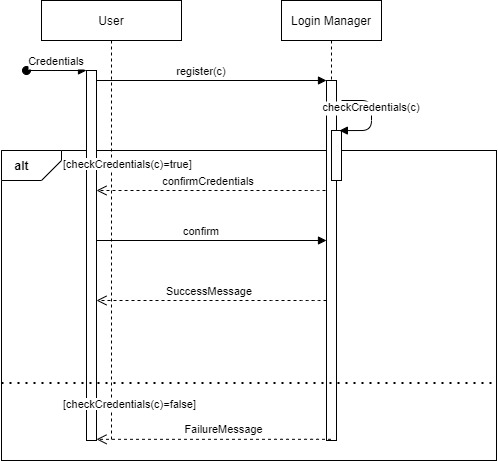
\includegraphics[height=0.5\textheight, scale=1, keepaspectratio]{img/seq_diag/Register.jpg}
            \captionof{figure}{Registration Sequence diagram, if the User confirms the credentials when they have to.}
\end{minipage}

\begin{minipage}{\linewidth}
            \centering
           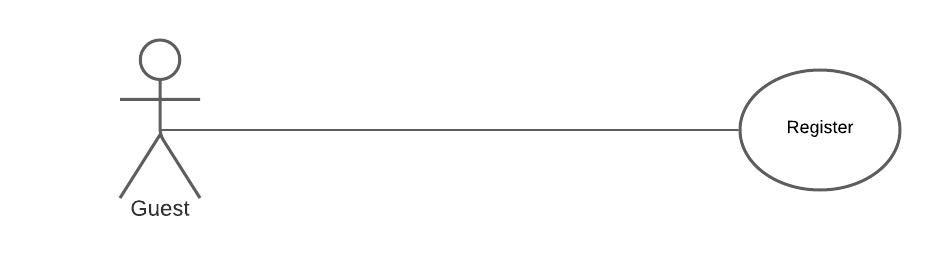
\includegraphics[height=0.1\textheight, scale=0.2, keepaspectratio]{img/registration_use_case_diagram.png}
            \captionof{figure}{Registration}
\end{minipage}

\begin{center}
{\textbf{\ref{uc:login}: Login}}
\end{center}
\begin{tabularx}{\linewidth}{| l | X |}
	%\hline
	%\textbf{ID} & \ref{uc:registration}\\
	
	\hline
	\textbf{Description} & A Customer wants to log-in into the main application.\\
	
	% \hline
	% \textbf{Achieved Goals} & {}\\

	\hline
	\textbf{Actors} & \textbf{\textit{Customer}}, \textbf{\textit{Login Manager}}\\
	
	\hline
	\textbf{Preconditions} & The Customer opens the application on their device and is registered.\\
	
	\hline
	\textbf{Flow of Events} & \parbox{0.7\textwidth}{	
		\begin{enumerate}
			\item The Customer fills the editable fields with the requested information: email and password
			\item The Customer clicks on the Sign In button.
			\item The Login Manager checks if the credentials are valid. 
			\item If the credentials are valid, the Customer successfully logs-in the application.
	\end{enumerate}}\\
	
	\hline
	\textbf{Post-Conditions} & The Customer logs-in the application with their personal account.\\
	
	\hline
	\textbf{Exceptions} & \parbox{0.7\textwidth}{ \begin{enumerate}
			\item If the Customer does not enter valid credentials, a failure message pops up on the screen prompting them to re-enter the credentials.
		\end{enumerate}}\\

	\hline
	
\end{tabularx}

\begin{minipage}{\linewidth}
            \centering
           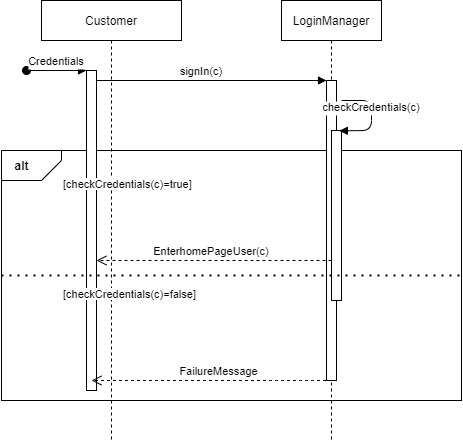
\includegraphics[height=0.5\textheight, scale=1, keepaspectratio]{img/seq_diag/Login.jpg}
            \captionof{figure}{Login Sequence diagram}
\end{minipage}

\begin{center}
{\textbf{\ref{uc:updateCredentials}: Update Credentials}}
\end{center}
\begin{tabularx}{\linewidth}{| l | X |}
	%\hline
	%\textbf{ID} & \ref{uc:registration}\\
	
	\hline
	\textbf{Description} & A Customer wants to update their credentials.\\
	
	% \hline
	% \textbf{Achieved Goals} & {}\\

	\hline
	\textbf{Actors} & \textbf{\textit{Customer}} and \textit{\textbf{Login Manager}}\\
	
	\hline
	\textbf{Preconditions} & The Customer opens the application on their device and is logged in.\\
	
	\hline
	\textbf{Flow of Events} & \parbox{0.7\textwidth}{	
		\begin{enumerate}
			\item The Customer clicks on the update credential button, from the home page\lorenzo{CHECK INTERFACES}.
			\item The Customer fills the editable fields with the requested information: email and password, and confirms the operation through a button.
			\item The Login Manager checks if the new credentials are valid. 
			\item If the new credentials are valid, the Customer has successfully updated their credentials
	\end{enumerate}}\\
	
	\hline
	\textbf{Post-Conditions} & The Customer successfully updates their credentials.\\
	
	\hline
	\textbf{Exceptions} & \parbox{0.7\textwidth}{ \begin{enumerate}
			\item If the Customer does not enter valid credentials, a failure message pops up on the screen, and the credentials are not updated.
		\end{enumerate}}\\

	\hline
	
\end{tabularx}

\begin{center}
{\textbf{\ref{uc:lostPassword}: Lost Password}}
% TODO
\end{center}
\begin{tabularx}{\linewidth}{| l | X |}
	%\hline
	%\textbf{ID} & \ref{uc:registration}\\
	
	\hline
	\textbf{Description} & A Customer wants to log-in into the main application but they have forgotten the password.\\
	
	% \hline
	% \textbf{Achieved Goals} & {}\\

	\hline
	\textbf{Actors} & \textbf{\textit{Customer}}, \textit{\textbf{Login Manager}}, \textit{\textbf{Mailing System}} \\
	
	\hline
	\textbf{Preconditions} & The Customer opens the application on their device and is registered.\\
	
	\hline
	\textbf{Flow of Events} & \parbox{0.7\textwidth}{	
		\begin{enumerate}
			\item The Customer clicks on the Recover Password button, in the log-in page \lorenzo{CHECK INTERFACES}.
			\item The Customer enter their mail in the editable box, and they click the recover password button.
			\item The Login Manager checks if the mail is associated to a registered Customer.
			\item If the mail is associated to a registered Customer, the Login Manager sends a mail to the user with appropriate instructions.
			\item The Customer follows the instructions on the email and is able to access their account.
	\end{enumerate}}\\
	
	\hline
	\textbf{Post-Conditions} & The Customer can log-in the application.\\
	
	\hline
	\textbf{Exceptions} & \parbox{0.7\textwidth}{ \begin{enumerate}
			\item If the Customer does not enter a mail associated to a registered user, the procedure fails and a failure message pops up on the screen, prompting the User to insert a mail associated to one account.
		\end{enumerate}}\\

	\hline
	
\end{tabularx}

\begin{center}
{\textbf{\ref{uc:getTicket}: Get Ticket}}
\end{center}
\begin{tabularx}{\linewidth}{| l | X |}
	%\hline
	%\textbf{ID} & \ref{uc:registration}\\
	
	\hline
	\textbf{Description} & A Customer requests a Virtual Ticket for lining up for entering a specific Store.\\
	
	% \hline
	% \textbf{Achieved Goals} & {}\\

	\hline
	\textbf{Actors} & \textbf{\textit{Customer}}, \textit{\textbf{Ticket Manager}}, \textit{\textbf{Queue Manager}} \lorenzo{Check These}\\
	
	\hline
	\textbf{Preconditions} & The Customer opens the application on their device and is logged in.\\
	
	\hline
	\textbf{Flow of Events} & \parbox{0.7\textwidth}{	
		\begin{enumerate}
		    \item The Customer clicks on the reservation tab in the home page.
			\item The Customer searches for the Store they want to go to, typing its name in the apposite text box or looking at the suggestions in the apposite list.
			\item The Customer clicks on the Store they want to go to, from the list which has spawned in the mean time.
			\item The Customer checks the Ticket check-box.
			\item The Customer specifies the duration of their Visit using the apposite GUI elements. The Customer can either input a duration or select one which is inferred by the DataAnalytics Manager.
			\item The Customer specifies with which means of transport they will go to the Store.
			\item Using third party API, and the current location of the Customer, the System compute how much time the Customer needs to go to the Store
			\item The Customer clicks on the get Ticket Button and the Ticket is sent to the Ticket Manager of the Store.
			\item The Ticket Manager checks if the information on the ticket is sound.
			\item The Ticket Manager sends the information on the Ticket to the Queue Manager of the Store, that looks for the available positions in the queue.
			\item The Queue Manager places the Customer in the queue accordingly and sends the information to the Ticket Manager.
			\item The System alerts the Customer on how much time they would have to wait for their turn and asks for confirmation.
			\item If the Customer clicks on the "reserve" button, and has no other valid ticket, the ticket request is successful and the ticket is reserved.
	\end{enumerate}}\\
	
	\hline
	\textbf{Post-Conditions} & The Customer gets the ticket.\\
	
	\hline
	\textbf{Exceptions} & \parbox{0.7\textwidth}{ \begin{enumerate}
			\item If the Customer exits the application before hitting the reserve button, the request is silently discarded (The Ticket Manager sends a message to the Queue Manager which deletes the Ticket from the queue).
			\item If there are no position available in the Queue, the system logs to the Customer a failure message and the request is discarded.
			\item If the Customer is too far away from the store to arrive and finish their shopping in time for the closure of the Store, the system logs to the User a failure message the request is discarded.
			\item If a Customer already has a Virtual Ticket in his reservations, the System does not allow the Customer to get another one, logs a failure message and the request is discarded.
			\item If the Customer takes too long to click the "reserve" button, the Ticket is cancelled.
		\end{enumerate}}\\

	\hline
	
\end{tabularx}

\begin{minipage}{\linewidth}
            \centering
           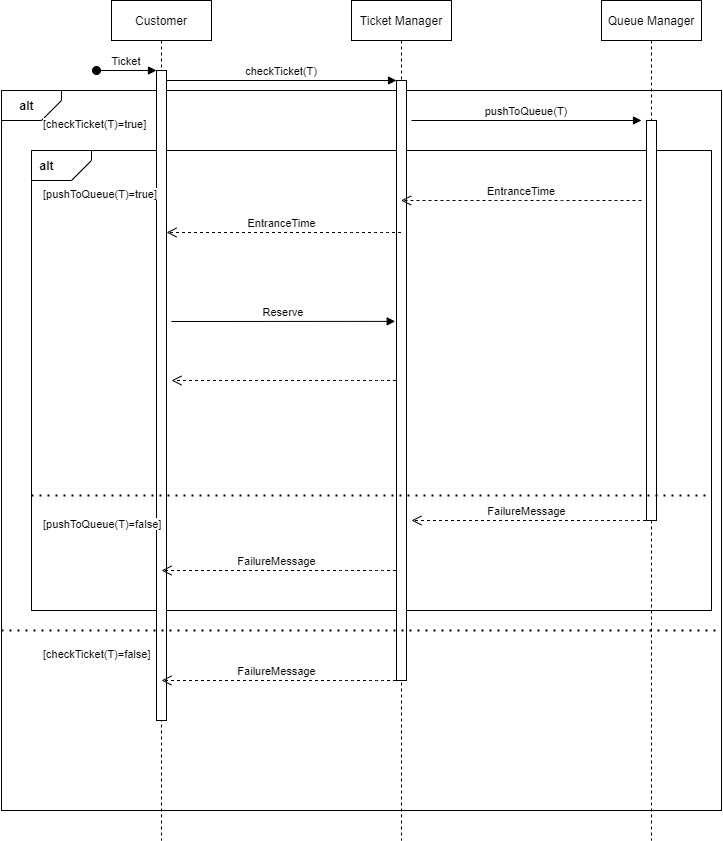
\includegraphics[height=0.5\textheight, scale=1, keepaspectratio]{img/seq_diag/GetTicket.jpg}
            \captionof{figure}{Get Ticket Sequence diagram, after having compiled the ticket form, and with the Customer clicking the reserve button respecting its time constraint.}
\end{minipage}

\begin{center}
{\textbf{\ref{uc:getVisit}: Book Visit}}
\end{center}
\begin{tabularx}{\linewidth}{| l | X |}
	%\hline
	%\textbf{ID} & \ref{uc:registration}\\
	
	\hline
	\textbf{Description} & A Customer books a Visit for a specific Store.\\
	
	% \hline
	% \textbf{Achieved Goals} & {}\\

	\hline
	\textbf{Actors} & \textbf{\textit{Customer}}, \textit{\textbf{Queuing mechanism}}, \textbf{\textit{Store Manager}}\lorenzo{CHECK THESE}\\
	
	\hline
	\textbf{Preconditions} & The Customer opens the application on their device and is logged in.\\
	
	\hline
	\textbf{Flow of Events} & \parbox{0.7\textwidth}{	
		\begin{enumerate}
			\item The Customer searches for the Store they want to go to, typing its name in the apposite text box or looks at the suggestions in the list.
			\item The Customer clicks on the Store they want to go to, from the list which has spawned in the mean time.
			\item The Customer checks the Visit check-box.
			\item The Customer specifies the duration of their Visit using the apposite GUI elements. The Customer can either input a duration or select one which is inferred by the Data Analytics Manager.
			\item The Customer specifies which day they are planning to do the Visit.
			\item Clicking the apposite button, the Customer sends the Visit to the Visit Manager of the Store.
			\item The Visit Manager checks if the information is valid and sends to the Queue Manager of the specified Store the Visit information.
			\item The Queue Manager sends the available time slots in the specified day to the Customer.
			\item The System displays time slots available, in the day requested by the Customer to visit the specific Store. The Customer can choose one of those.
			\item The Customer can select the categories of items they would like to buy.
			\item The Customer can book the Visit, clicking on the apposite button, if in the specified day they do not have already booked 3 Visits.
			\item The Customer sends the Visit information directly to the appropriate Queue Manager and this inserts the Customer into the Queue of the Store, in the specified day, and at the specified time.
	\end{enumerate}}\\
	
	\hline
	\textbf{Post-Conditions} & The Customer books the Visit.\\
	
	\hline
	\textbf{Exceptions} & \parbox{0.7\textwidth}{ \begin{enumerate}
			\item If the Customer has booked three Visits in specified day, the system logs a failure message and discards the Visit.
			\item If there are not any available time-slots (of any Store) the System logs a failure message.
			\item If, when the Customer sends the confirmation of the booking, the time-slot selected is not available anymore, the System logs an error message.
		\end{enumerate}}\\

	\hline
	
\end{tabularx}

\begin{minipage}{\linewidth}
            \centering
           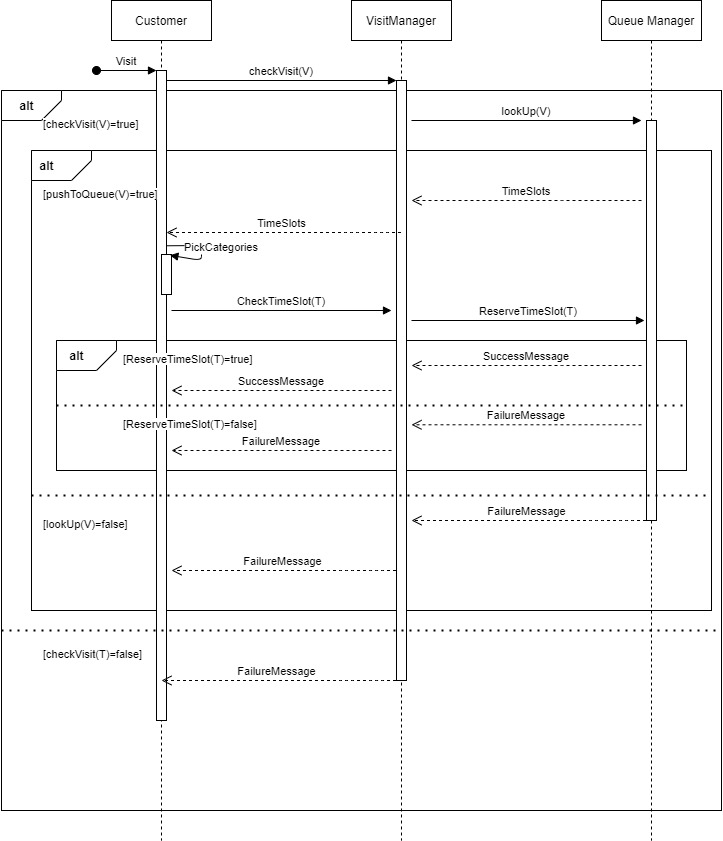
\includegraphics[height=0.5\textheight, scale=1, keepaspectratio]{img/seq_diag/GetVisitD.jpg}
            \captionof{figure}{Book Visit Sequence diagram, after having compiled the Visit form.}
\end{minipage}

\begin{minipage}{\linewidth}
        \centering
           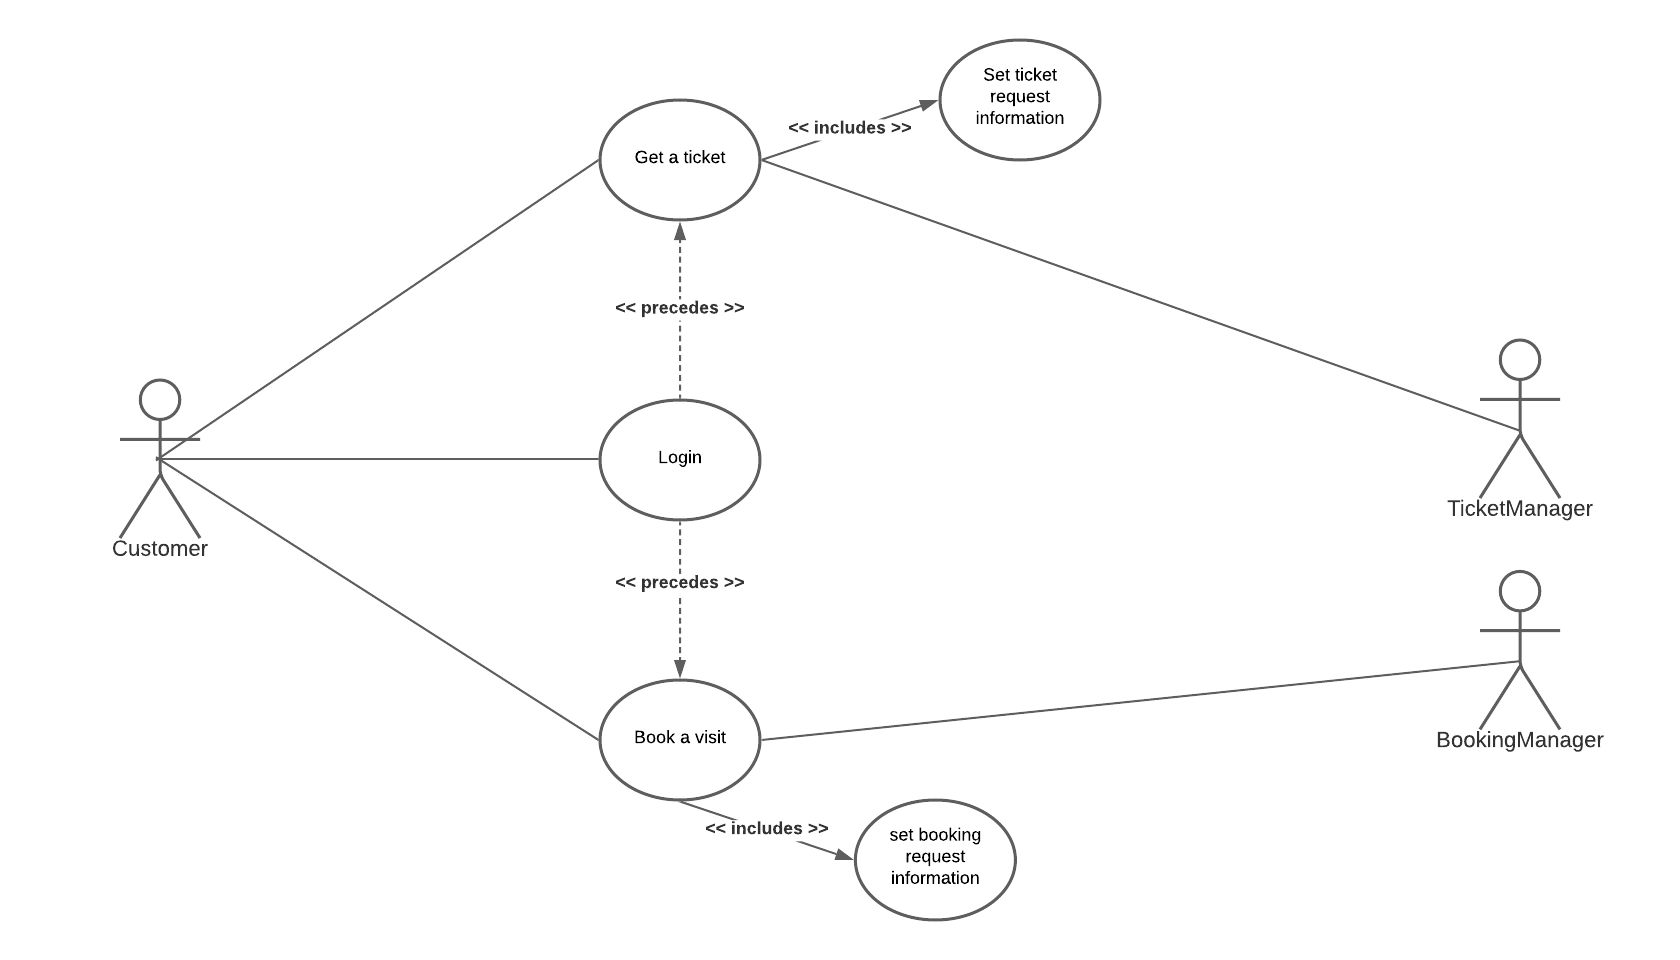
\includegraphics[height=0.4\textheight, scale=0.1, keepaspectratio]{img/book_ticket_use_diagram.png}
            \captionof{figure}{Get Ticket and Book Visit}
        \end{minipage}

\begin{center}
{\textbf{\ref{uc:accessStore}: Access Store - Using Ticket}}
\end{center}
\begin{tabularx}{\linewidth}{| l | X |}
	%\hline
	%\textbf{ID} & \ref{uc:registration}\\
	
	\hline
	\textbf{Description} & A Customer shops into a store, accessing it with a ticket.\\
	
	% \hline
	% \textbf{Achieved Goals} & {}\\

	\hline
	\textbf{Actors} & \textbf{\textit{Customer}}, \textit{\textbf{Queue Manager}}  \lorenzo{CHECK THESE}\\
	
	\hline
	\textbf{Preconditions} & The Customer has a reserved ticket.\\
	
	\hline
	\textbf{Flow of Events} & \parbox{0.7\textwidth}{	
		\begin{enumerate}
			\item The System tells the Customer when to depart from their place to go to the Store on time with the specified means of transport.
			\item Once arrived at the Store the Customer checks the entrance time on the Ticket (it could be updated). The Customer enters the Store when specified by the ticket.
			\item The Customer scans their personal QR-code (which can be found in the profile tab in the app) with the Machine for Scanning provided by the Store.
			\item The Customer enters the Store and tries to comply with the duration specified on the ticket.
			\item The system collects the duration of the shopping, storing it in the Database \lorenzo{CHECK THIS}.
			\item If the Customer takes more time to shop than the duration specified, the Queue Manager applies a scaling process to avoid overcrowding.
			\item After paying the Customer is prompted by the Store's operator to scan again the QR-code.
	\end{enumerate}}\\
	
	\hline
	\textbf{Post-Conditions} & The Customer has done their shopping in the desired Store.\\
	
	\hline
	\textbf{Exceptions} & \parbox{0.7\textwidth}{ \begin{enumerate}
			\item If the Customer cannot make it in time, the ticket reserved is invalidated by the Queue Manager.
		\end{enumerate}}\\

	\hline
	
\end{tabularx}

\begin{center}
{\textbf{\ref{uc:accessStore}: Access Store - Using Visit}}
\end{center}
\begin{tabularx}{\linewidth}{| l | X |}
	%\hline
	%\textbf{ID} & \ref{uc:registration}\\
	
	\hline
	\textbf{Description} & A Customer shops into a store, accessing it with a Visit.\\
	
	% \hline
	% \textbf{Achieved Goals} & {}\\

	\hline
	\textbf{Actors} & \textbf{\textit{Customer}}, \textit{\textbf{Queue Manager}}  \\
	
	\hline
	\textbf{Preconditions} & The Customer has a valid Visit booked.\\
	
	\hline
	\textbf{Flow of Events} & \parbox{0.7\textwidth}{	
		\begin{enumerate}
			\item Once arrived at the Store the Customer checks the entrance time on the Visit they booked (it could be updated). The customer enters the Store when specified by the Visit.
			\item The Customer scans their personal QR-code (which can be found in the profile tab in the app) with the machine provided by the Store.
			\item The Customer enters the Store and tries to comply with the duration specified on the ticket.
			\item If the Customer is late, the Queue Manager automatically updates the queue to avoid overcrowding.
			\item The Customer is guided by the app through the store thanks to a map which show them the path to arrive to the categories specified during the booking of the Visit.
			\item The system collects the duration of the Visit, storing it in the Database \lorenzo{CHECK THIS}.
			\item After paying the Customer is prompted by the Store's operator to scan again the QR-code.
	\end{enumerate}}\\
	
	\hline
	\textbf{Post-Conditions} & The Customer has done their Visit in the desired Store.\\
	
	\hline
	\textbf{Exceptions} & \parbox{0.7\textwidth}{ \begin{enumerate}
			\item If the Customer cannot make it in time, the ticket reserved is invalidated by the Queue Manager.
		\end{enumerate}}\\

	\hline
\end{tabularx}

\begin{center}
{\textbf{\ref{uc:deleteBooked}: Delete Booked}}
\end{center}
\begin{tabularx}{\linewidth}{| l | X |}
	%\hline
	%\textbf{ID} & \ref{uc:registration}\\
	
	\hline
	\textbf{Description} & A Customer deletes a booked Visit or a Ticket.\\
	
	% \hline
	% \textbf{Achieved Goals} & {}\\

	\hline
	\textbf{Actors} & \textbf{\textit{Customer}}, \textit{\textbf{Queue Manager}}  \lorenzo{CHECK THESE}\\
	
	\hline
	\textbf{Preconditions} & The Customer has booked a Visit or reserved a Ticket.\\
	
	\hline
	\textbf{Flow of Events} & \parbox{0.7\textwidth}{	
		\begin{enumerate}
			\item The Customer goes onto the reservation tab.
			\item The Customer presses onto the reservation they want to delete.
			\item The Customer presses on the delete button.
			\item The Queue Manager receives a notification with the information of the reservation.
			\item The Queue Manager deletes the reservation.
			\item The Queue Manager updates the queue status accordingly.
	\end{enumerate}}\\
	
	\hline
	\textbf{Post-Conditions} & The Customer has deleted their Visit/Ticket reservation.\\
	
	\hline
	\textbf{Exceptions} & \parbox{0.7\textwidth}{ \begin{enumerate}
			\item During the Visit/shopping time with the Ticket, the Costumer cannot delete the corresponding Ticket/Visit.
		\end{enumerate}}\\

	\hline
\end{tabularx}


\begin{center}
{\textbf{\ref{uc:createStore}: Create Store}}
\end{center}
\begin{tabularx}{\linewidth}{| l | X |}
	%\hline
	%\textbf{ID} & \ref{uc:registration}\\
	
	\hline
	\textbf{Description} & A Manager creates a new Store.\\
	
	% \hline
	% \textbf{Achieved Goals} & {}\\

	\hline
	\textbf{Actors} & \textbf{\textit{Manager}}, \textit{\textbf{Mailing Service}}  \lorenzo{CHECK THESE}\\
	
	\hline
	\textbf{Preconditions} & The Manager is logged-in into the main application. \\
	
	\hline
	\textbf{Flow of Events} & \parbox{0.7\textwidth}{	
		\begin{enumerate}
			\item The Manager clicks on the create Store button in the store tab.
			\item The Manager inputs the requested information in the editable boxes.
			\item The Manager inputs special credentials, (PEC email associated to the Store), to certify the authenticity of the Store. \lorenzo{CHECK THIS}
			\item The Customer follows the instructions on the email to activate the Store.
			\item The System sends an email to the given PEC to finalize the Store creation.
			\item The Store is created, and the Manager becomes the Owner of the Store.
	\end{enumerate}}\\
	
	\hline
	\textbf{Post-Conditions} & The Store is created, and the Manager becomes the Owner of the Store.\\
	
	\hline
	\textbf{Exceptions} & \parbox{0.7\textwidth}{ \begin{enumerate}
			\item If the information given is invalid, the System denies the Store creation and logs to the screen an error message.
		\end{enumerate}}\\

	\hline
\end{tabularx}

\begin{center}
{\textbf{\ref{uc:useScanner}: Activate Scanner}}
\end{center}
\begin{tabularx}{\linewidth}{| l | X |}
	%\hline
	%\textbf{ID} & \ref{uc:registration}\\
	
	\hline
	\textbf{Description} & A Manager activates a scanner associated with one of their Stores.\\
	
	% \hline
	% \textbf{Achieved Goals} & {}\\

	\hline
	\textbf{Actors} & \textbf{\textit{Manager}}, \textit{\textbf{Queuing Manager}}\\
	
	\hline
	\textbf{Preconditions} & The Manager opens the application on their device and is associated to a Store.\\
	
	\hline
	\textbf{Flow of Events} & \parbox{0.7\textwidth}{	
		\begin{enumerate}
			\item The Manager clicks on the interested Store
			\item The Manager clicks on the generate scanner button
			\item The System generates a unique code, the scanner code associated with the Queue Manager of the Store.
			\item The Manager can send this code to their clerks/machines.
			\item The clerks with the code can access a specific application and input it in the specific editable text box.
			\item The clerks can now use this app to scan the QR-codes of the Customers.
			\item Each scan can influence the queue status.
	\end{enumerate}}\\
	
	\hline
	\textbf{Post-Conditions} & The Store is able to scan the tickets of the Customers.\\
	
	\hline
	\textbf{Exceptions} & \parbox{0.7\textwidth}{ \begin{enumerate}
			\item If the code input in the app is wrong, the System outputs a failure message on the screen.
		\end{enumerate}}\\

	\hline
	
\end{tabularx}

\begin{center}
{\textbf{\ref{uc:usePaper}: Activate Paper Ticket}}
\end{center}
\begin{tabularx}{\linewidth}{| l | X |}
	%\hline
	%\textbf{ID} & \ref{uc:registration}\\
	
	\hline
	\textbf{Description} & A Manager activates a paper-ticket service associated with one of their Stores.\\
	
	% \hline
	% \textbf{Achieved Goals} & {}\\

	\hline
	\textbf{Actors} & \textbf{\textit{Manager}}, \textit{\textbf{Queue Manager}}\\
	
	\hline
	\textbf{Preconditions} & The Manager opens the application on their device and is associated to a Store.\\
	
	\hline
	\textbf{Flow of Events} & \parbox{0.7\textwidth}{	
		\begin{enumerate}
			\item The Manager clicks on the interested Store
			\item The Manager clicks on the generate paper ticket button
			\item The System generates a unique code, the paper-ticket code associated with the queue of the Store.
			\item The Manager can use this code in the apposite machine, to set up a paper ticket service
			\item The Consumers can now get tickets from this machine.
			\item Each tickets influences the queue status.
	\end{enumerate}}\\
	
	\hline
	\textbf{Post-Conditions} & The Store is able to produce paper tickets for the Consumers.\\
	
	\hline
	\textbf{Exceptions} & \parbox{0.7\textwidth}{ \begin{enumerate}
			\item If the code input in the app is wrong, the System outputs a failure message on the screen.
		\end{enumerate}}\\

	\hline
	
\end{tabularx}

\begin{center}
{\textbf{\ref{uc:updateStoreInfo}: Update Store Info}}
\end{center}
\begin{tabularx}{\linewidth}{| l | X |}
	%\hline
	%\textbf{ID} & \ref{uc:registration}\\
	
	\hline
	\textbf{Description} & A Manager wants to update Store information.\\
	
	% \hline
	% \textbf{Achieved Goals} & {}\\

	\hline
	\textbf{Actors} & \textbf{\textit{Manager}}, \textit{\textbf{Queue Manager}}\\
	
	\hline
	\textbf{Preconditions} & The Manager opens the application on their device and is associated to a Store.\\
	
	\hline
	\textbf{Flow of Events} & \parbox{0.7\textwidth}{	
		\begin{enumerate}
			\item The Manager clicks on the interested Store
			\item The Manager clicks on the update information\lorenzo{CHECK INTERFACES}.
			\item The Manager fills the editable fields with the updated information and confirms the operation through a button. (Simple Manager and Owner, have different editable fields).
			\item If the Manager has edited information which are linked to the Queue Manager (max number of people, opening hours, amount of days in advance in which a Visit can be booked), the System logs a message: these changes can be uploaded within 24 hours, taking a chance on canceling some Visits previously booked, or can be uploaded in the current amount of days in advance in which a Visit can be booked, without losing any Visit.
			\item The Queue Manager handles the changing of the information linked to the queue in the due time.
			\item The System sends notifications to Customers if their Visits have been cancelled.
	\end{enumerate}}\\
	
	\hline
	\textbf{Post-Conditions} & The Manager successfully updates the Store information.\\
	
	\hline
	\textbf{Exceptions} & \parbox{0.7\textwidth}{ \begin{enumerate}
			\item If the Manager inputs some invalid information, the operation fails and is cancelled and the System logs a failure message on the screen.
		\end{enumerate}}\\

	\hline
	
\end{tabularx}

\section{Formal Analysis Using Alloy}
This section is dedicated to the description of the model through the use of the Alloy modeling language, which allows us to describe the world in which our application lives.

\subsection{World Generated: main characteristics}
In the Figure \ref{alloy_world} it is possible to observe the main aspects of the System and its relations. In order to show also the details of the world, the various components will be examined separately in the next sections.
\begin{figure}[h!]
\centering
	\centering
  	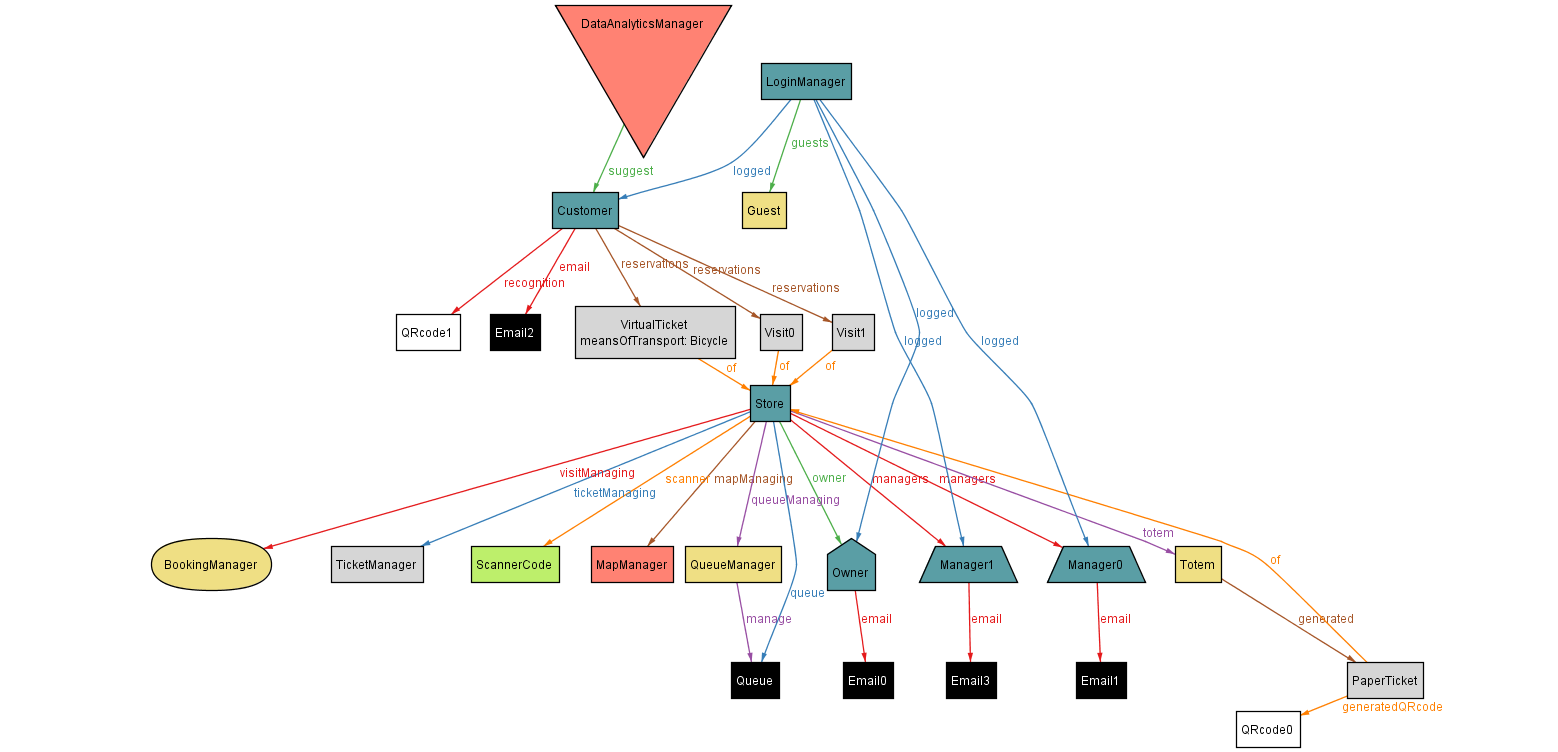
\includegraphics[height=0.32\textheight, scale=0.3, keepaspectratio]{img/alloy/alloy_world.png}
	\caption{Alloy-generated world that shows the most important interactions.}
 	\label{alloy_world}
\end{figure}

\subsubsection{Login Manager and Data Analytics Manager}
The Login Manager is in charge of providing the login functionality. 
each Guest must enter their login credentials to interface with the app features. A logged in User can be a Manager or a Customer. Each User has its own personal Email. Each Customer is identified by his personal unique QRCode, and has his own Reservations. Moreover, each Customer 
will receive suggestions from the Data Analytics Manager, which is in charge of analyze data about Customers. All this details are shown in the Figure \ref{alloy_login}.
\begin{figure}[h!]
\centering
	\centering
  	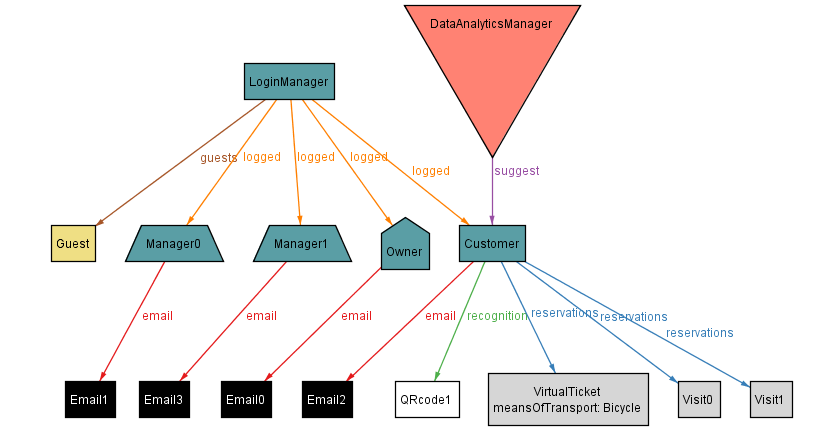
\includegraphics[height=0.32\textheight, scale=0.3, keepaspectratio]{img/alloy/alloy_login_manager.png}
	\caption{Alloy-generated world that shows the Login Manager and the Data Analytics Manager functionalities.}
 	\label{alloy_login}
\end{figure}

\subsubsection{Customers and their Reservations}
As we can see in the Figure \ref{alloy_customer} Customers are identified by a unique QRCode. Each Customer can have some Reservations planned, which can be a Visi or a VirtualTicket. Every Visit is characterized by the Day of the Visit, the TimeSlot for that Visit, a List of Groceries that the Customer wants to buy and a Duration.  Each VirtualTicket is chacterized by a time of entrance and a duration. Moreover each Reservation refers to one Store. A single Customer cannot reserve more than 3 Visits in the same Day for the same Store.
\begin{figure}[h!]
\centering
	\centering
  	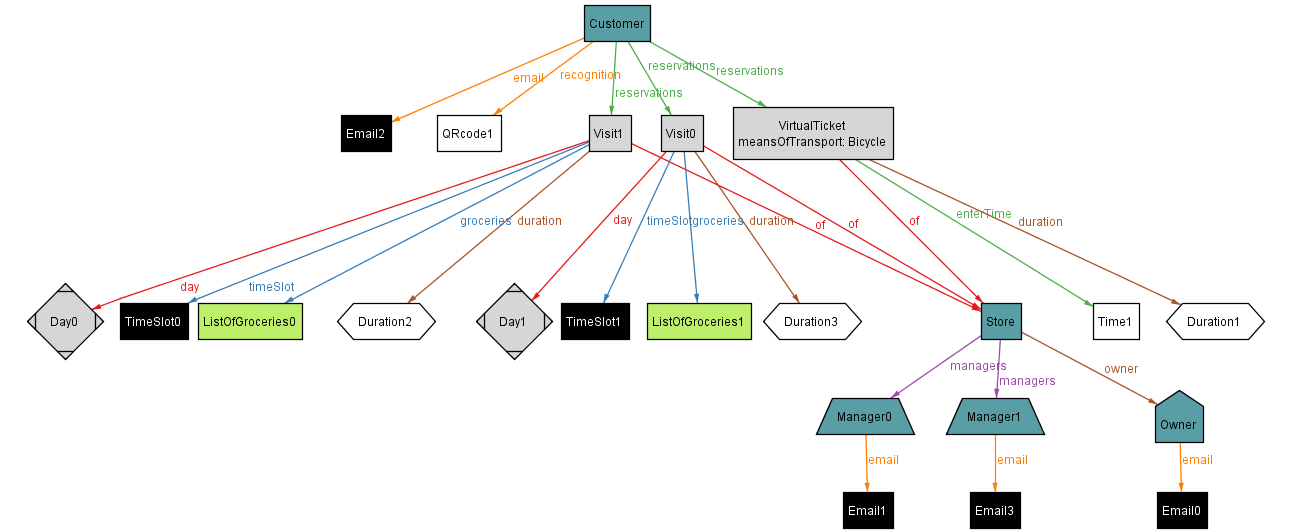
\includegraphics[height=0.27\textheight, scale=0.3, keepaspectratio]{img/alloy/alloy_customer_reservations.png}
	\caption{Alloy-generated world that shows Customers and Reservations characteristics.}
 	\label{alloy_customer}
\end{figure}

\subsubsection{Stores and their components}
Each Store has one and only one Owner, but it can have other Managers who collaborate in the management of the Store. Moreover each Store has its own BookingManager, TicketManager and MapManager. This components are made in order to manage all the requests of Tickets and Visits for that Store. It also has a ScannerCode and a Totem. The Totem has the task of generating PaperTickets for that particular Store, which will be characterized by a unique QRcode. The Reservations made for a Store are stored in the personal unique Queue of the Store, which is managed by the Queue Manager. A Queue has a certain number of Temporal Quantums, and each Temporal Quantum has a number of spaces equal to the capacity of the Store.
\begin{figure}[h!]
\centering
	\centering
  	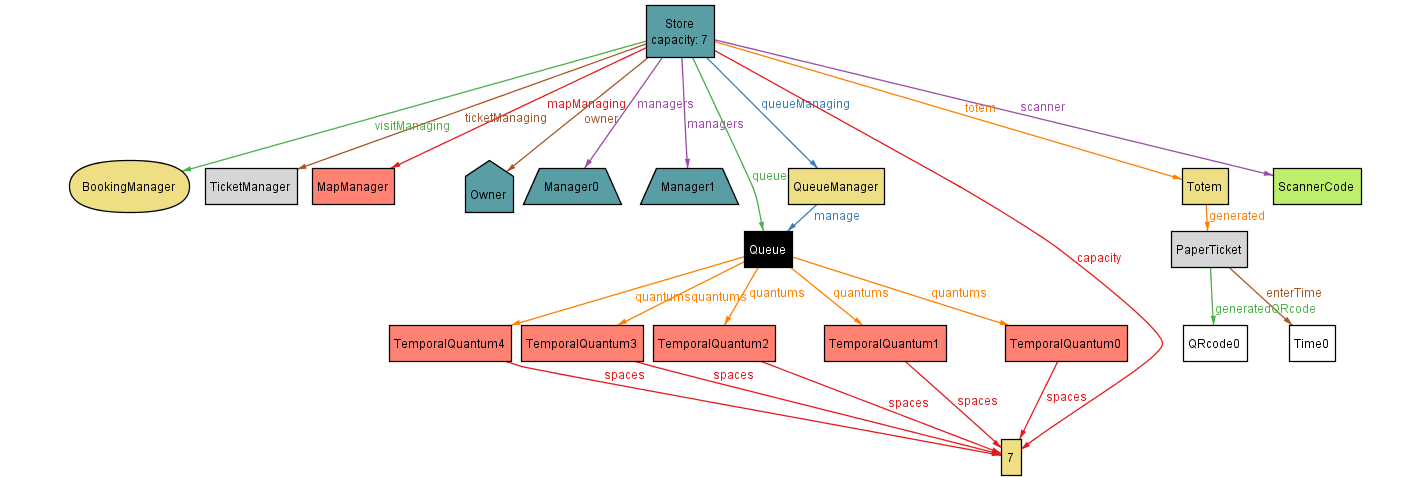
\includegraphics[height=0.23\textheight, scale=0.3, keepaspectratio]{img/alloy/alloy_store.png}
	\caption{Alloy-generated world that shows Customers and Reservations characteristics.}
 	\label{alloy_customer}
\end{figure}

\subsubsection{The Whole World Generated}
\begin{figure}[h!]
\centering
	\centering
  	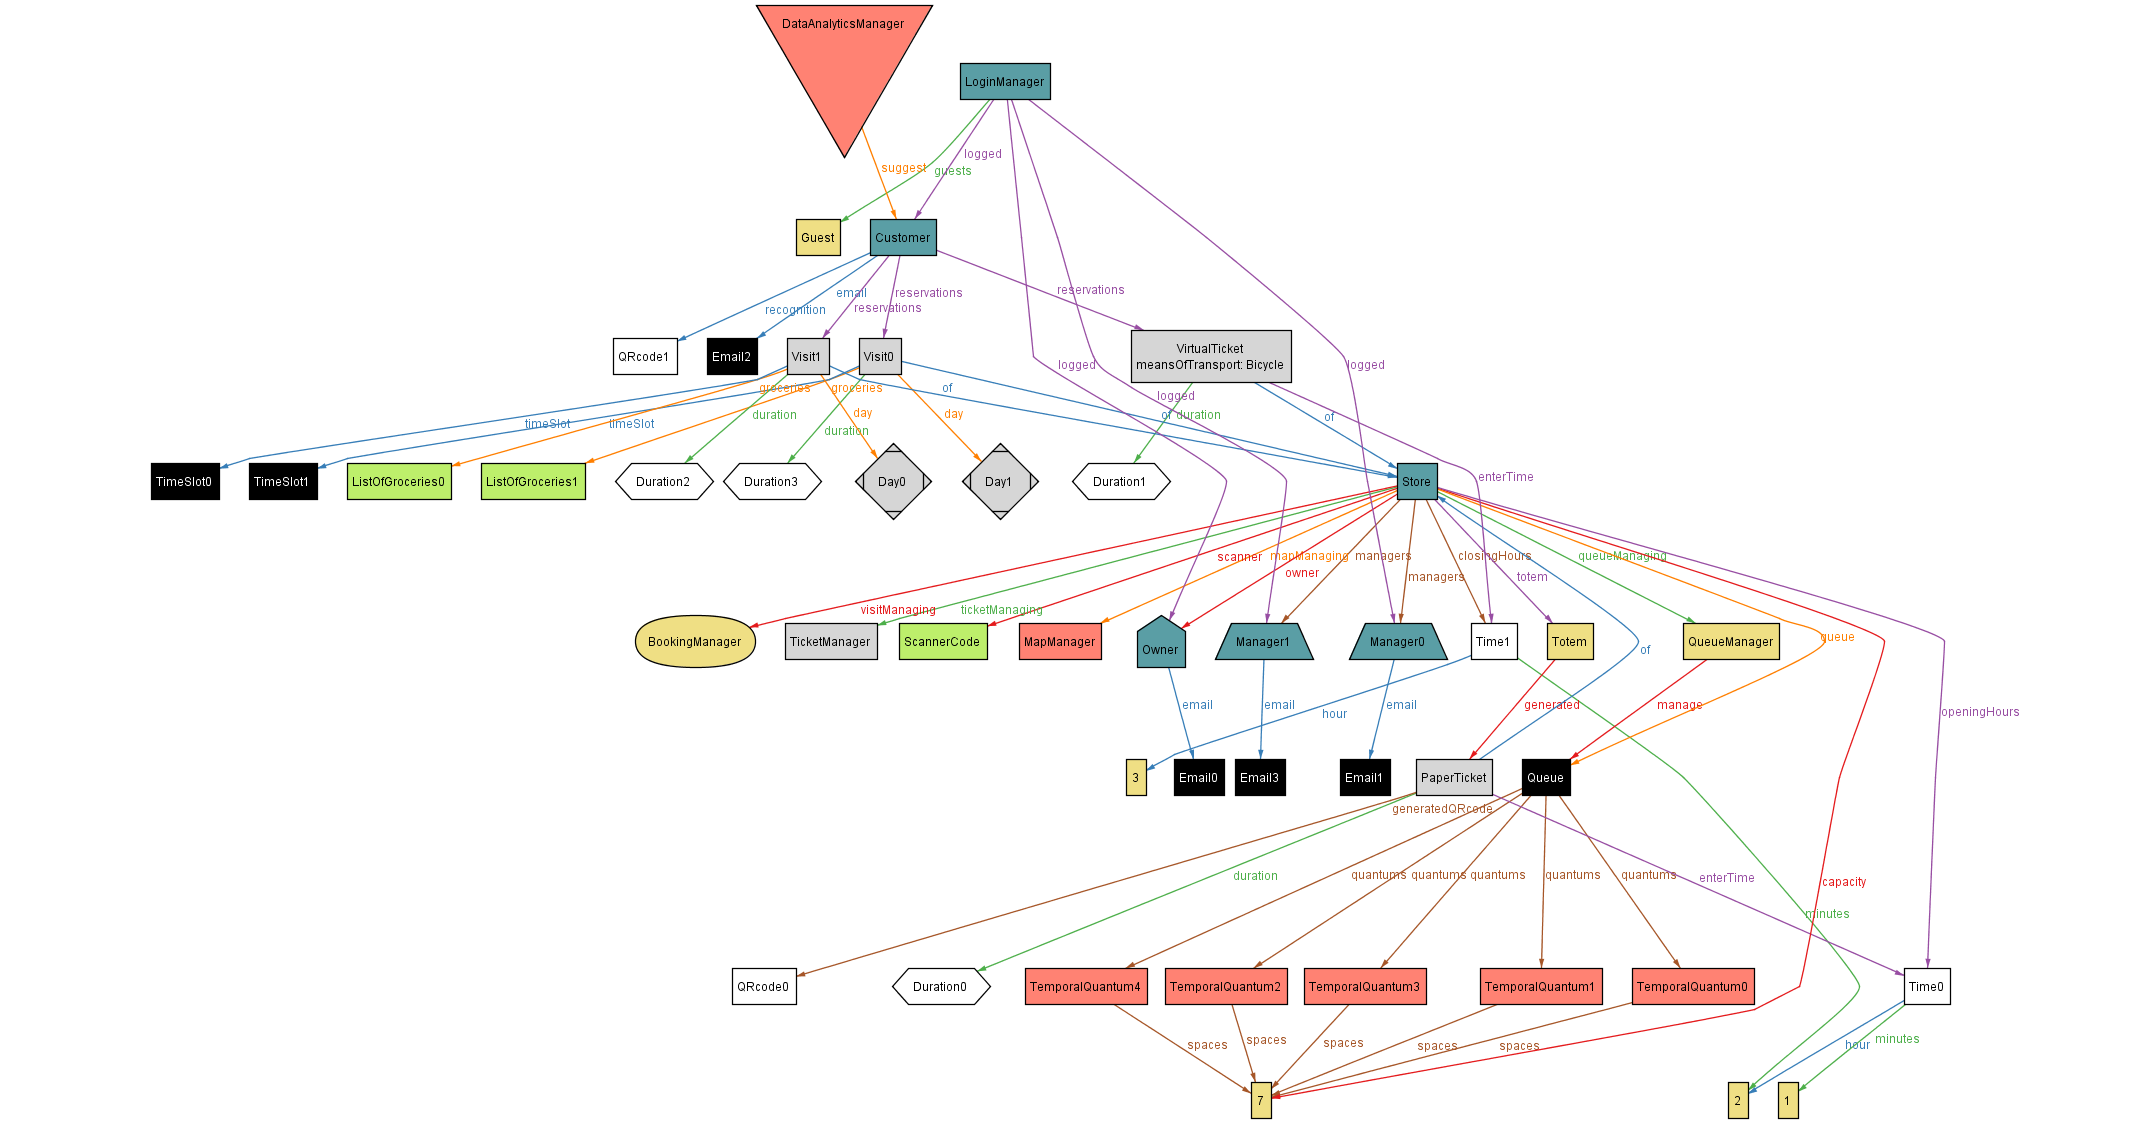
\includegraphics[height=0.35\textheight, scale=0.3, keepaspectratio]{img/alloy/alloy_entire_world.png}
	\caption{Alloy-generated entire world.}
 	\label{alloy_entire_world}
\end{figure}

In Figure \ref{alloy_entire_world} there is the representation of the whole world generated by Alloy, by running the following predicate: 

\begin{lstlisting}[language=alloy]
pred show{
	#Guest = 1
	#Queue = 1
	#TemporalQuantum = 5
	#Totem = 1
	#ScannerCode = 1
	#Manager = 3
	#Visit = 2
	#VirtualTicket = 1
	#PaperTicket = 1
	#Customer = 1
	#DataAnalyticsManager = 1
	#LoginManager = 1
}

run show for 20
\end{lstlisting}

\subsection{Model Check}
\begin{lstlisting}[language=alloy]
-- All VirtualTickets and Visits belong to a Customer, all PaperTickets are generated by a Totem --
assert noAloneReservations{
	all vt:VirtualTicket | one c:Customer {
		vt in c.reservations
	}
	all v:Visit | one c:Customer{
		v in c.reservations
	}
	all pt:PaperTicket | one t:Totem{
		pt in t.generated
	}
}

-- There are no more than 3 Visits per day for only one Customer --
assert maxThreeVisitPerDayForACustomer{
	all d:Day | all c:Customer | #(c.reservations & day.d) <= 3
}

-- Each Email is of one and only one User and is unique for each User --
assert uniqueEmail{
	all disj u1,u2:User | u1.email != u2.email
	all u:User | #u.email = 1
}
 
-- Unique QR code --
assert uniqueQRcode{
	//There are no QRCodes in common between Customers and PaperTickets
	all disj c:Customer | all disj pt:PaperTicket { c.recognition != pt.generatedQRcode }
	//Each PaperTicket has a unique QRcode
	all disj c1,c2:Customer | c1.recognition != c2.recognition
	//Each Customer has a unique QRcode
	all disj p1,p2:PaperTicket | p1.generatedQRcode != p2.generatedQRcode
}

-- Capacity and number of spaces in each TemporalQuantum of a Store --
assert capacityAndSpaces{
	all s:Store | s.capacity = s.queue.quantums.spaces
}

-- Unique Components for each Store --
assert componentsStore{
	all s:Store | #(s.ticketManaging) = 1 && #(s.visitManaging) = 1 && #(s.queueManaging) = 1 && #(s.mapManaging) = 1
}

-- Each Queue is of one and only one Store and is unique for each Store --
assert uniqueQueue{
	all disj s1,s2:Store | s1.queue != s2.queue
	all s:Store | #s.queue = 1	
}

-- Each Store has only one Owner --
assert oneOwner{
	all s:Store | #s.owner = 1
}
\end{lstlisting}

The results of the running of all the assertions above can be found in the Figure \ref{check_alloy}. As you can see, no counterexample has been found.

\begin{figure}[hbt]
\centering
\begin{subfigure}
	\centering
  	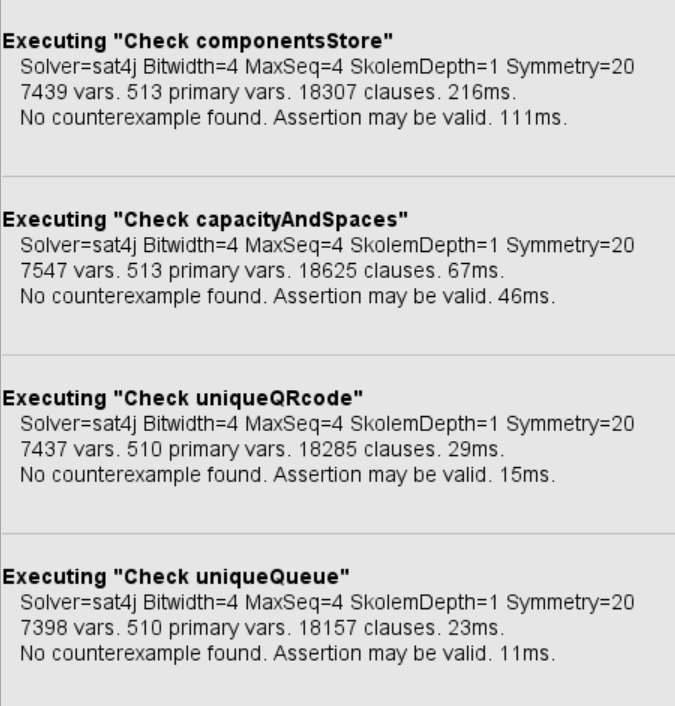
\includegraphics[height=0.3\textheight, scale=0.2, keepaspectratio]{img/alloy/img_check_1.PNG}
 \end{subfigure}
 \begin{subfigure}
	\centering
  	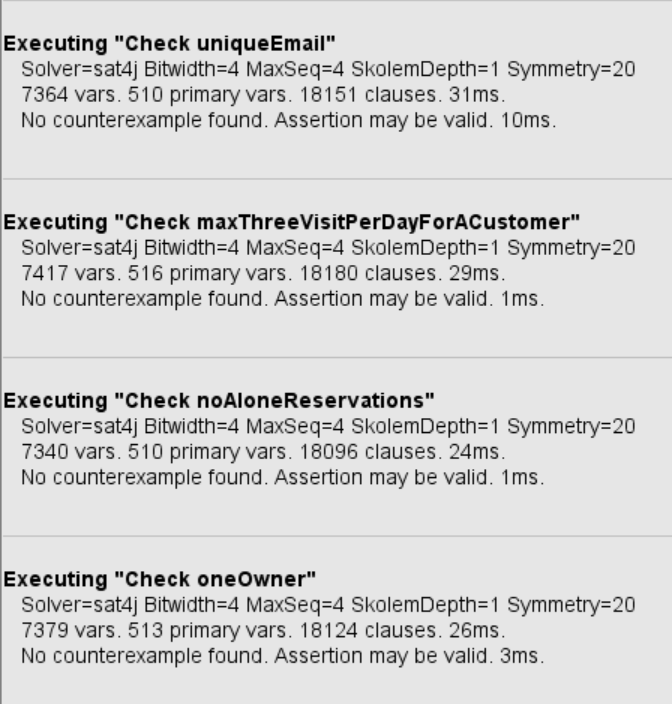
\includegraphics[height=0.3\textheight, scale=0.2, keepaspectratio]{img/alloy/img_check_2.PNG}
 \end{subfigure}
	\caption{Results for running all the assertions made. No counterexample has been found.}
 	\label{check_alloy}
\end{figure}

\subsection{Whole Alloy Model}
\begin{lstlisting}[language=alloy]
-- SIGNATURES AND FACTS --
abstract sig MeansOfTransport { }
one sig Car extends MeansOfTransport { }
one sig Walk extends MeansOfTransport { }
one sig PublicMeans extends MeansOfTransport { }
one sig Bicycle extends MeansOfTransport { }

one sig LoginManager{
	logged: some User, 
	guests: some Guest
}

one sig DataAnalyticsManager{
	suggest: set Customer
 }{
	(#DataAnalyticsManager > 0) <=> (#Customer > 0)
}

sig TicketManager{ }{
	one s:Store | this in s.ticketManaging
}

sig BookingManager{ }{
	one s:Store | this in s.visitManaging
}

sig QueueManager{
	manage: one Queue
 }{
	one s:Store | this in s.queueManaging
}

sig MapManager{ }{
	one s:Store | this in s.mapManaging
}

sig  Duration{ }{
	//Each Duration belongs to a Reservation
	one r:Reservation | this in r.duration
}

sig ListOfGroceries{ }{
	//Each ListOfGroceries belongs to a Visit
	one v:Visit | this in v.groceries
	//All Visits have different ListOfGroceries
	all disj v1,v2:Visit | v1.groceries != v2.groceries
}

sig Day{ }{
	//Each Day belongs to a Reservation
	one r:Reservation | this in r.day
}

sig TimeSlot{ }{
	//Each TimeSlot belongs to at least one Visit
	one v:Visit | this in v.timeSlot
}

sig Time{
	hour: one Int,
	minutes: one Int
}{
	hour >= 0
	hour < 24
	minutes >= 0
	minutes < 60
}

sig Char{ }{
	//Each Char belongs to an email
	one e:Email | this in e.email
}

sig Guest { }{
	//Each Guest has to be managed by a LoginManager
	one lm:LoginManager | this in lm.guests
}

//Email as a sequence of char
sig Email{
     email: seq Char
}{
	//Each Email belongs to a User
	one u:User | this in u.email
}

sig QRcode{ }{
	//Each QRcode belongs to a Customer or to a PaperTicket
	one c:Customer | one pt:PaperTicket{
		this in c.recognition || this in pt.generatedQRcode
	}
	//There are no QRcode in common
	all disj c:Customer | all disj pt:PaperTicket{ 
		#(c.recognition & pt.generatedQRcode)=0 
	}
	all disj p1,p2:PaperTicket | p1.generatedQRcode != p2.generatedQRcode
	all disj c1,c2:Customer | c1.recognition != c2.recognition
}

abstract sig Reservation { 
	duration: one Duration,
	of: one Store
}

abstract sig Ticket extends Reservation{
	enterTime: one Time
}

sig PaperTicket extends Ticket {
	generatedQRcode: one QRcode
}{
	// Each Ticket is associate to one and only one Consumer
	one t:Totem | this in t.generated
}

sig VirtualTicket extends Ticket {
	meansOfTransport: one MeansOfTransport
}{
	// Each VirtualTicket is associate to one and only one Customer
	one c:Customer | this in c.reservations
}

sig Visit extends Reservation {
	day: one Day,
	timeSlot: one TimeSlot,
	groceries: one ListOfGroceries
}{
	// Each Visit is associated to one and only one Customer
	one c:Customer | this in c.reservations
}

sig ScannerCode {}{
	//Each ScannerCode is of a Store
	one s:Store | this in s.scanner
}

sig Queue {
	quantums: some TemporalQuantum
} {
	// Foreach queue, each quantum has the same spaces
	all q1, q2: quantums | q1.spaces =q2.spaces
	// Each queue has to be associated to one and only one Store
	one s:Store | this = s.queue
	//queueManager of the Store manage manage only the queue of the that Store
	all s:Store | s.queueManaging.manage = s.queue
}

/*sig Consumer {
	reservations: some Reservation
}*/

abstract sig User { 
	email: one Email
}{
	//Each User has to be logged by a LoginManager
	one lm:LoginManager | this in lm.logged
}

sig Customer extends User{
	reservations: some Reservation,
	recognition: one QRcode,
	/*password: one String*/
}{
	// each customer has at most 3 visits each day
	all d:Day | #(reservations & day.d) <= 3
	//each customer receives suggestions from the DataAnalyticsManager
	all d:DataAnalyticsManager | this in d.suggest
}

//Check that no one has an email used by another Customer
fact emailUnique{
	all u, u1: User |  (u.email = u1.email) iff (u = u1)
}



sig Manager extends User {}{
	one s:Store | this in s.managers || this in s.owner 
}

sig Owner extends Manager {}{
	// Each owner associated to a one and only one Store
	one s:Store | this =s.owner
}

sig Store {
	owner: one Owner,
	managers: set Manager,
	scanner: one ScannerCode,
	totem: some Totem,
	capacity: one Int,
	queue: one Queue,
	openingHours: one Time,
	closingHours: one Time,
	ticketManaging: one TicketManager,
	visitManaging: one BookingManager,
	queueManaging: one QueueManager,
	mapManaging: one MapManager
}{
	// Queue available places equal to the capacity of the associated store (for each store)
	queue.quantums.spaces = capacity
	// for each store capacity has to be greater than 0
	capacity > 0
	// For each Store, the owner is not also a manager.
	owner not in managers
	// Each store must close after opening
	openingHours.hour < closingHours.hour
}

sig TemporalQuantum{
	spaces: one Int	
}{
	// Each Temporal quantum is associated to one and only queue
	one q:Queue.quantums | this = q
}

sig Totem {
	generated: set PaperTicket
}{
	//Each Totem is of a Store
	one s:Store | this in s.totem
}


-- ASSERTIONS --

-- All VirtualTickets and Visits belong to a Customer, all PaperTickets are generated by a Totem --
assert noAloneReservations{
	all vt:VirtualTicket | one c:Customer {
		vt in c.reservations
	}
	all v:Visit | one c:Customer{
		v in c.reservations
	}
	all pt:PaperTicket | one t:Totem{
		pt in t.generated
	}
}

-- There are no more than 3 Visits per day for only one Customer --
assert maxThreeVisitPerDayForACustomer{
	all d:Day | all c:Customer | #(c.reservations & day.d) <= 3
}

-- Each Email is of one and only one User and is unique for each User --
assert uniqueEmail{
	all disj u1,u2:User | u1.email != u2.email
	all u:User | #u.email = 1
}
 
-- Unique QR code --
assert uniqueQRcode{
	//There are no QRCodes in common between Customers and PaperTickets
	all disj c:Customer | all disj pt:PaperTicket { c.recognition != pt.generatedQRcode }
	//Each PaperTicket has a unique QRcode
	all disj c1,c2:Customer | c1.recognition != c2.recognition
	//Each Customer has a unique QRcode
	all disj p1,p2:PaperTicket | p1.generatedQRcode != p2.generatedQRcode
}

-- Capacity and number of spaces in each TemporalQuantum of a Store --
assert capacityAndSpaces{
	all s:Store | s.capacity = s.queue.quantums.spaces
}

-- Unique Components for each Store --
assert componentsStore{
	all s:Store | #(s.ticketManaging) = 1 && #(s.visitManaging) = 1 && #(s.queueManaging) = 1 && #(s.mapManaging) = 1
}

-- Each Queue is of one and only one Store and is unique for each Store --
assert uniqueQueue{
	all disj s1,s2:Store | s1.queue != s2.queue
	all s:Store | #s.queue = 1	
}

-- Each Store has only one Owner --
assert oneOwner{
	all s:Store | #s.owner = 1
}


-- PREDICATE --

pred show{
	#Guest = 1
	#Queue = 1
    	#TemporalQuantum = 5
	#Totem = 1
	#ScannerCode = 1
	#Manager = 3
	#Visit = 2
	#VirtualTicket = 1
	#PaperTicket = 1
	#Customer = 1
	#DataAnalyticsManager = 1
	#LoginManager = 1
}


-- EXECUTION --

run show for 20
\end{lstlisting}

\section{Effort Spent}
\label{effort}
sample effort spent

\section{REFERENCES}
\label{references}
\renewcommand{\refname}{}
\vspace{-2.6em}
\nocite{*}
\bibliography{biblio} 
\bibliographystyle{unsrtnat}

\end{document}
